\documentclass[pdflatex,sn-basic]{sn-jnl}

\usepackage{graphicx}
\graphicspath{{./}{../figures_pdf_vector/}}
\usepackage{multirow}
\usepackage{amsmath,amssymb,amsfonts}
\usepackage{amsthm}
\usepackage[title]{appendix}
\usepackage{xcolor}
\usepackage{textcomp}
\usepackage{manyfoot}
\usepackage{booktabs}
\usepackage{listings}
\usepackage{array}

\lstset{basicstyle=\ttfamily\footnotesize, breaklines=true,
        columns=fullflexible, frame=none}

\newcommand{\researchq}[1]{\textbf{RQ#1}}

\raggedbottom

\begin{document}

\title[Boundary-Mutation Testing for Secret Detection]{Boundary-Mutation Testing for Pattern-Based Secret Detection: A Rule-Level Method and a 774-Type, Three-Scanner Evaluation}

\author*[1]{\fnm{Shweta} \sur{Mishra}}\email{shweta.mishra.research@gmail.com}
\equalcont{ORCID: 0009-0002-8443-1678}

\affil*[1]{\orgname{Independent Researcher}, \orgaddress{\city{Moradabad}, \country{India}}}

\abstract{Secret scanners are validated with example-based fixtures that fix one variable: the text surrounding a credential. Boundary-mutation testing varies it: credentials are generated from each rule's own regular expression, embedded in realistic source contexts, and judged at the rule level, yielding three detection metrics. We apply it to a 43-rule open-source scanner, Gitleaks 8.21.2 and TruffleHog 3.82.13: on ten shared credential types, then on 774 types generated from all three tools' rule tables. Every tool has a boundary defect. In the primary subject a final hyphen drops detection from $\geq$0.9976 to 0.5233; we trace it to a word-boundary anchor and validate a repair, after a plausible first repair regressed two rules. Gitleaks' terminator allowlist misses a credential followed by `)' for 159 of the 218 types it covers. TruffleHog, robust on the ten shared types, misses hyphen-terminated credentials for 91 of the 117 types whose formats allow them --- a conclusion the small study had inverted. Of seventeen further contexts, base64 hides every self-identifying credential from two tools, and a split string defeats all three for most types. On 9.87 million lines from 31 repositories in nine languages, 28.9\% of credential-shaped tokens outside test, documentation and fixture paths are followed by a character Gitleaks rejects. Scale changes the comparison: ten types support no ranking, but on types generated by neither tool in a pair, the primary subject --- the author's own --- covers fewer types than either alternative ($p=0.0004$; $p=2.5\times10^{-7}$) and has the highest false-positive rate on the nine-language corpus.}

\keywords{secret detection, credential leakage, mutation testing, metamorphic testing, regular expressions, empirical software engineering}

\maketitle

\section{Introduction}

Credential leakage through source repositories is a persistent and largely preventable security failure~\citep{meli2019}. The standard control is a pattern-based secret scanner: a table of regular expressions, usually paired with an entropy heuristic, applied to diffs or working trees. Gitleaks~\citep{gitleaks}, TruffleHog~\citep{trufflehog}, GitHub's hosted secret scanning, and the scanner studied here all belong to this family.

Such rule tables are commonly validated with example-based fixtures. A contributor adding a rule writes one or two credentials of the new shape into a test file and asserts they are detected; the scanner we study validates 43 rules with a 313-line fixture suite, and the practice is visible in the test suites of the other two tools as well. We do not claim to have surveyed the field exhaustively, and we do not need to: the weakness we identify follows from the structure of example-based fixtures, not from their prevalence.

That weakness is this. A regular expression does not match a credential in isolation; it matches a credential \emph{together with its surroundings}, and anchoring assertions such as \verb|\b| take effect precisely at the join between the two. Hand-written fixtures almost always place the credential in one canonical position --- inside a double-quoted assignment, ending in an alphanumeric character. A rule that fails only when a credential is passed as a bare function argument, or only when its final character happens to be a hyphen, cannot be observed by a suite in which no fixture is written that way.

This paper introduces \emph{boundary-mutation testing} to vary that surrounding context systematically. Three design choices distinguish it from writing more test cases. First, credentials are generated from \emph{each rule's own regular expression}, so the corpus is derived from the artefact under test rather than from the experimenter's intuitions. Second, each credential is embedded in a battery of contexts, each one a way a credential legitimately appears in real source. Third --- and this is what makes the defects visible --- outcomes are classified at the \emph{rule} level, distinguishing ``the credential's own rule fired'' from ``something fired'' (Fig.~\ref{fig:framework}). The gap between those two is where a severity downgrade hides, and a tool-level binary metric cannot see it.

\begin{figure}[t]
\centering
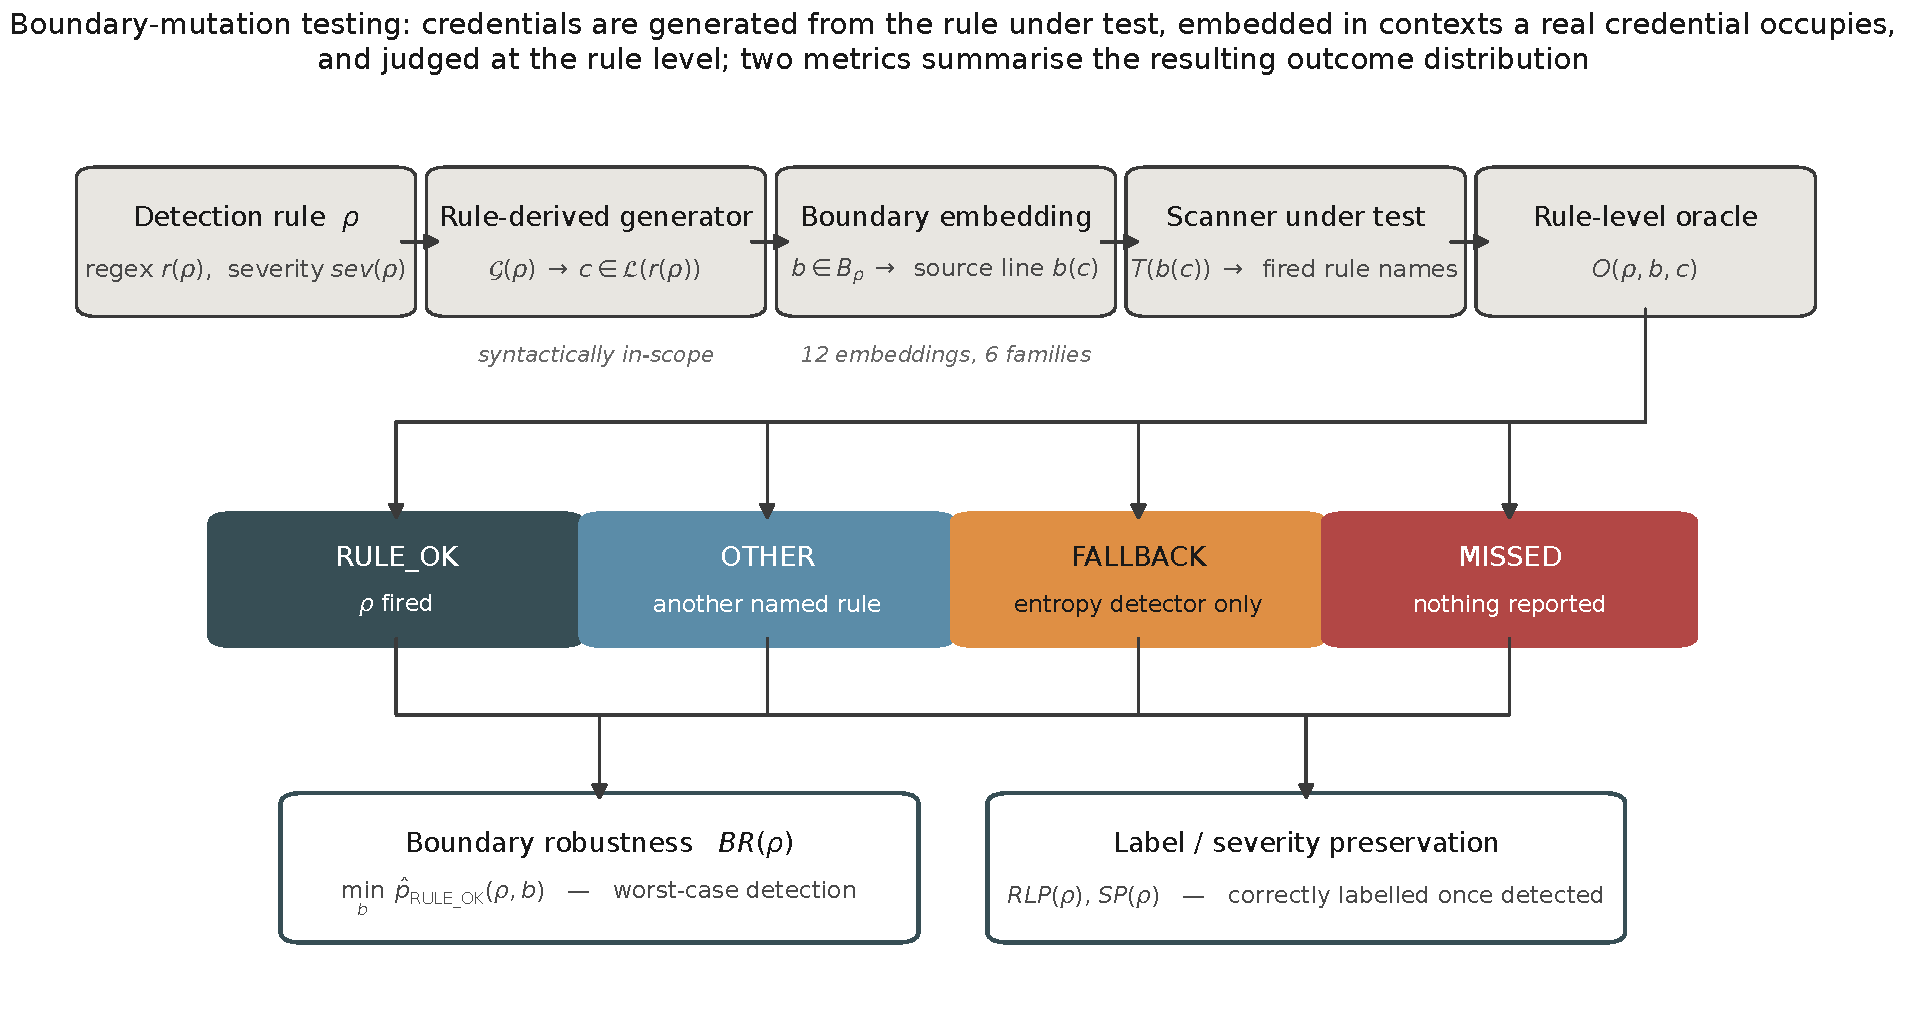
\includegraphics[width=\textwidth]{fig00_framework.pdf}
\caption{Boundary-mutation testing. A credential is generated from the rule under test, embedded in a context that a real credential of that type occupies, and the outcome is classified at the rule level. The four outcome classes yield the three metrics of Section~\ref{sec:metrics}.}
\label{fig:framework}
\end{figure}

We apply the method at two scales. On the primary subject's own rules and ten credential types shared by three independent scanners, it finds and explains a defect, and validates a repair. It then scales without change to the tools' full rule tables: 774 credential types, generated from the rule tables of all three tools, are run through all three (Section~\ref{sec:scale}). The two scales disagree, and the disagreement is itself a result. At ten types one scanner appears boundary-robust and the comparison is underpowered; at 774 types every scanner has a boundary defect, and a comparison on types generated by neither tool in a pair resolves an ordering --- one that runs against the raw ten-type numbers and against the primary subject, which is the author's own. We report the mechanism behind each defect, the marginal (not merely conditional) probability that it affects a credential, how often the contexts that trigger it occur in 9.87 million lines of real code in nine languages, and how the tools handle credentials that are escaped, interpolated, marked up or transformed rather than merely bounded.

\medskip\noindent\textbf{Contributions.}
\begin{enumerate}
\item \textbf{A method and three metrics.} Boundary-mutation testing, formally defined as a family of metamorphic relations (Section~\ref{sec:method}), with \emph{boundary robustness} $BR(\rho)$, \emph{rule-label preservation} $RLP(\rho)$ and \emph{severity preservation} $SP(\rho)$ derived from its outcome classification.
\item \textbf{Mechanisms, not just findings.} Each defect is traced to a specific regular-expression construct and confirmed on minimal pairs, with marginal failure probabilities computed under an explicitly stated model (Sections~\ref{sec:rq2} and~\ref{sec:rq3}).
\item \textbf{A validated repair, and a caution about validating repairs.} We patch the five defective rules of the primary subject, re-run the full battery, and confirm $BR=1.0$ with no new false positives on real code. A first candidate patch, plausible on inspection, is shown by the same battery to regress two rules to total failure on a case the original rule handled correctly (Section~\ref{sec:repair}).
\item \textbf{Evidence at the scale of full rule tables.} Applied to 774 types from all three rule tables, the battery finds a boundary defect in every tool (Section~\ref{sec:rq3}): Gitleaks' terminator allowlist defeats 159 of the 218 types it covers on a single context, a defect we confirm from its published configuration; TruffleHog's word-boundary anchors defeat 91 of 117 types on a trailing hyphen, contrary to the ten-type result; and two Gitleaks rules miss any unquoted token followed by a line break, a defect we have not seen reported.
\item \textbf{Beyond the boundary.} Seventeen further contexts in five families --- escaping, interpolation, markup, file syntax and transformed values --- separate the defects that follow from boundary handling from those that follow from what a tool decodes (Section~\ref{sec:rq6}).
\item \textbf{Real-code exposure, not only synthetic rates.} On 31 commit-pinned repositories in nine languages, we measure false positives on one identical file set for all tools, and how often credential-shaped tokens of any provider stand in a context the measured defects depend on (Sections~\ref{sec:rq5}--\ref{sec:rq6}).
\item \textbf{Benchmark design as a measured confound.} Corpus construction, deployment condition, the number of credential types, and which tool generated them each change what a comparison reports (Section~\ref{sec:rq4}). At ten types no difference is significant; at 774, with generator bias controlled, the ordering is significant and reverses the one the ten-type numbers suggested.
\end{enumerate}

\medskip\noindent\textbf{Scope.} This is a methods paper about rule-level detection. Two subsystems of the primary subject are therefore deliberately excluded from the main study. Its LLM layer is unmeasured because no funded provider credential was available (Section~\ref{sec:notmeasured}). Its operational characteristics --- queueing, concurrency, and fault tolerance --- were separately characterised and are reported in Online Resource~1; they are outside the scope of the research questions and bear on none of the claims made here.

\medskip\noindent\textbf{Research contribution versus engineering artefact.} Because one of the three evaluated systems is the author's own, we state this distinction explicitly rather than leave it implicit. The \emph{research contribution} is boundary-mutation testing itself: the method, its formalisation as a family of metamorphic relations, its three derived metrics, and the empirical evidence in Sections~\ref{sec:rq1}--\ref{sec:repair} about boundary-sensitive detector behaviour, obtained by applying that method to three independently developed systems. GitHub Autopilot is an \emph{engineering artefact} used to instantiate and validate the methodology --- one experimental subject among three, not the paper's object of study. Nothing in our claims depends on which of the three subjects it is; Section~\ref{sec:bias} details the controls taken because it happens to be ours.

\section{Research Questions}

\noindent\researchq{1} \emph{Does rule-level detection depend on the source context surrounding a credential, and which contexts degrade it?}

\noindent\researchq{2} \emph{What mechanism produces any context sensitivity found, and what is the marginal probability that it affects a real credential?}

\noindent\researchq{3} \emph{Does the method transfer to independently developed scanners and to their full rule tables, and is the defect class shared or tool-specific?}

\noindent\researchq{4} \emph{How do the three scanners compare, and how much do corpus construction, deployment condition, the number of credential types and the choice of generator change that comparison?}

\noindent\researchq{5} \emph{What is the false-positive behaviour of each scanner on unmodified real code in nine languages?}

\noindent\researchq{6} \emph{How do the scanners handle credentials that are escaped, interpolated, marked up or transformed, and how often do credential-shaped tokens in real code stand in the contexts the boundary defects depend on?}

\section{Related Work}

\textbf{Secret detection.} \citet{meli2019} measured secret leakage on GitHub at scale, establishing that leaked credentials are common and long-lived. Subsequent work targets the false-positive burden that impedes adoption~\citep{saha2020,rahman2019}, and recent studies examine the accuracy of detection tooling in practice~\citep{basak2022}.

Two lines are especially close to ours and warrant an explicit comparison. \citet{basak2023comparative} evaluate nine open-source and proprietary secret detection tools against a benchmark corpus and report wide disagreement between them, particularly in precision; \citet{basak2023secretbench} contribute the benchmark dataset that makes such comparisons possible, drawn from secrets checked into public repositories. More recently, \citet{li2025android} evaluate checked-in secret detection for Android applications and likewise conclude that current techniques have substantial limitations. All three establish, from independent evidence, the premise this paper takes as its starting point: detection tools disagree, and their measured accuracy is sensitive to what they are measured against.

Our question is different in what it holds fixed. Those studies compare tools on a corpus of credentials collected or curated from the field, so the credential and its surrounding text vary together and the tool is the manipulated variable. We invert that. The credential is generated from the detector's own rule, and the \emph{context} surrounding it is the manipulated variable, so a change in outcome is attributable to the boundary rather than to the sample. Outcomes are then judged against a rule-level oracle rather than a tool-level verdict, which separates a miss from a detection carrying the wrong label and severity. That combination --- inputs generated from each artefact's own declared language, context as the treatment, and a rule-level oracle --- is what we have not found in prior work, and it is what allows the defects in Section~\ref{sec:rq3} to be traced to a specific regular-expression construct rather than reported as an aggregate accuracy difference. To the best of our knowledge, no prior study systematically varies the context surrounding a credential while attributing outcomes at the rule level, and we are not aware of prior reports of either defect in Section~\ref{sec:rq3}. Table~\ref{tab:relatedwork} positions this work against the closest related lines.

\textbf{Mutation and metamorphic testing.} Classical mutation testing perturbs the \emph{program} to assess a test suite~\citep{jia2011,demillo1978}. We invert this: the artefact under test is a rule table, and we perturb the \emph{input}. In that respect the method is metamorphic~\citep{chen2018metamorphic,segura2016}: our context mutations are metamorphic relations, since re-quoting a credential or moving it into a YAML file should not change whether it is a credential. The distinguishing elements here are that inputs are generated \emph{from the artefact's own rules}, and that the oracle is rule-level rather than output-level.

\textbf{Input generation and grammar-based testing.} Generating inputs from a formal description relates to grammar-based fuzzing~\citep{godefroid2008} and property-based testing~\citep{claessen2000}, where a generator produces values satisfying a specification. Our generator consumes the detector's own regular expressions, which makes the positive corpus definitionally in-scope for the rule being tested --- a miss cannot be dismissed as outside the rule's syntactic specification, though, as Section~\ref{sec:validity} sets out, syntactic scope is not the same as provider-semantic validity. Work on regular-expression correctness and behaviour~\citep{chapman2016,michael2019} documents that developers frequently misunderstand anchoring and character-class semantics; both defects we report are instances of exactly that, in security-critical rules.

\textbf{Benchmark design as a confound.} Evidence continues to accumulate that benchmark construction, not only technique quality, drives measured outcomes~\citep{liem2020,herbold2020}. Sections~\ref{sec:rq4}--\ref{sec:rq5} contribute three instances in which construction alone reorders tools.

\textbf{Evaluating security scanners.} A recurring finding in the evaluation of static security tools is that measured effectiveness is highly sensitive to the benchmark rather than to the tool: reported detection rates vary widely across corpora, and tools tuned to one benchmark generalise poorly to another. Our Sections~\ref{sec:rq4}--\ref{sec:rq5} are three instances of the same phenomenon in the secret-detection setting, with the additional observation that the sensitivity is large enough to reverse the ordering. Where that literature typically compares tools, we use the sensitivity itself as the object of study and decline to produce a ranking.

\textbf{The unit of analysis in tool comparison.} Our Section~\ref{sec:paired} rests on a point that is well established in empirical software engineering but easy to lose in tool evaluation: when outcomes are deterministic within a stratum, the stratum and not the individual sample is the independent observation. Treating 400 credentials drawn from 10 deterministic types as 400 observations inflates the evidence by the number of samples per type. We report the paired test at the type level for this reason, and consequently report a null result where the sample-level intervals would have suggested a clear ordering.

\begin{table}[t]
\centering
\caption{This work against the closest related testing methods.}
\label{tab:relatedwork}
\small
\setlength{\tabcolsep}{5pt}
\begin{tabular}{@{}p{5.6cm}ccccc@{}}
\toprule
Line of work & Scan. & Mut. & Meta. & Gen. & Oracle \\
\midrule
Secret-leakage \& FP studies~\citep{meli2019,saha2020,rahman2019,basak2022} & \checkmark & & & & \\
Comparative scanner evaluation on curated corpora~\citep{basak2023comparative,basak2023secretbench,li2025android} & \checkmark & & & & \\
Classical mutation testing~\citep{jia2011,demillo1978} & & \checkmark & & & \\
Metamorphic testing~\citep{chen2018metamorphic,segura2016} & & & \checkmark & & \\
Grammar-/property-based generation~\citep{godefroid2008,claessen2000} & & & & \checkmark$^{*}$ & \\
\textbf{This work} & \checkmark & \checkmark & \checkmark & \checkmark & \checkmark \\
\botrule
\end{tabular}
\vspace{2pt}

\raggedright\footnotesize
Scan.~=~evaluates a security scanner; Mut.~=~mutation testing; Meta.~=~metamorphic testing; Gen.~=~inputs generated from a formal rule/specification; Oracle~=~outcome judged at rule level. $^{*}$Generates from a formal specification, not from a detector's own rule. Regex-correctness studies~\citep{chapman2016,michael2019} motivate Sections~\ref{sec:rq2}--\ref{sec:rq3} but are an empirical study, not a method, so are cited in text only and omitted from the rows above.
\end{table}

\textbf{Standards and formats.} The defects reported here affect detection of JSON Web Tokens~\citep{rfc7519} and OAuth bearer credentials~\citep{rfc6749}, whose encodings determine the marginal probabilities of Section~\ref{sec:rq2}; the HMAC construction underlying JWT signatures is specified in~\citep{rfc2104}. Complexity~\citep{mccabe1976} and coverage~\citep{zhu1997coverage} appear only in the supplementary subject characterisation, and the resilience patterns exercised there are due to \citet{nygard2018release} and \citet{fowler2014circuitbreaker}. \citet{wessel2018bots} and \citet{vasilescu2015ci} study bots and CI at the process level; our subject is one such bot, but it is studied here only as the owner of a rule table.

\section{Subject Systems}

The unit of analysis throughout is a \emph{detection rule}, not a tool. We study three rule tables belonging to independently developed scanners.

The primary subject is the secret scanner of GitHub Autopilot, an open-source self-hosted GitHub App available at \url{https://github.com/Shweta-Mishra-ai/github-autopilot} and studied here at commit \texttt{38b2013}. Its scanner comprises 43 regular-expression rules with per-rule severities, plus one unanchored entropy fallback that fires on high-entropy strings no named rule claims. We make no claim about its deployment scale; it is studied because its rule table is open, small enough to characterise exhaustively, and structurally representative of the regex-plus-entropy family.

Fig.~\ref{fig:arch} places that scanner within the system it belongs to, and marks the scope of this study. The scanner is the primary object of study. The ingress pipeline, queue and worker pool are characterised in the supplementary artefact but are not the subject of any claim made here. The LLM routing layer is unmeasured entirely (Section~\ref{sec:notmeasured}).

\begin{figure}[t]
\centering
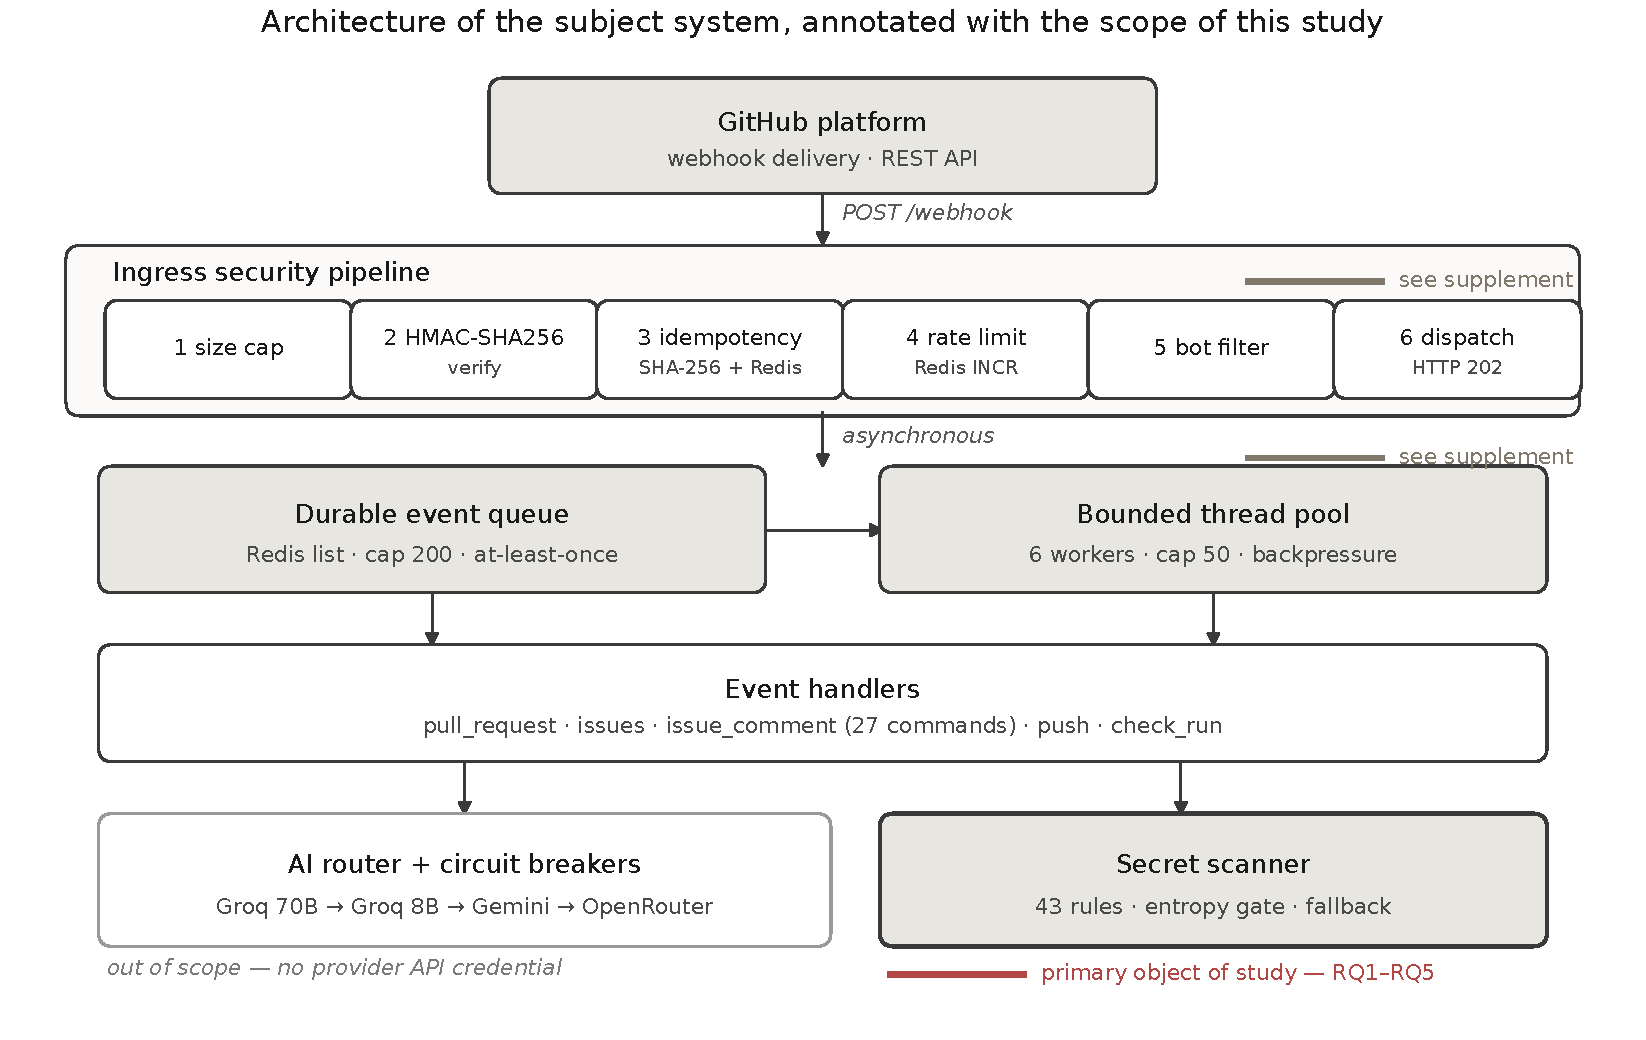
\includegraphics[width=\textwidth]{fig01_architecture.pdf}
\caption{The primary subject, annotated with the scope of this study. Only the secret scanner is the object of the research questions; the ingress and concurrency subsystems are characterised in the supplementary artefact, and the LLM routing layer is unmeasured.}
\label{fig:arch}
\end{figure}

Table~\ref{tab:subject} characterises the subject quantitatively. These measurements describe \emph{what was evaluated}; they are not evidence for or against the correctness of its scanner, and we do not treat them as results. They matter for two reasons only. First, they establish that the subject is a maintained system with a real test suite rather than a toy, which is what makes a defect in its rule table interesting. Second, they establish that its rule table is small enough to characterise exhaustively --- all 43 rules were examined, not a sample.

\begin{table}[t]
\centering
\caption{Characteristics of the primary subject at commit \texttt{38b2013}. Provided to characterise the experimental subject; not treated as evidence of scanner correctness.}
\label{tab:subject}
\small
\begin{tabular}{@{}lr@{}}
\toprule
Property & Value \\
\midrule
Application modules & 91 \\
Application lines of Python & 19{,}352 \\
Test lines of Python & 19{,}825 \\
Functions and methods & 617 \\
Mean cyclomatic complexity & 4.67 \\
Maximum cyclomatic complexity & 34 \\
\midrule
Test cases & 2{,}054 \\
Test outcome & 2{,}054 passing \\
Statement coverage & 83.9\% (7{,}600 statements) \\
Lint violations (\texttt{ruff}) & 0 \\
\midrule
Scanner rules & 43 named $+$ 1 entropy fallback \\
Rules analysed in this study & 24 (Section~\ref{sec:method}) \\
Scanner fixture suite & 313 lines \\
\botrule
\end{tabular}
\end{table}

The last two rows are the ones that motivate this paper. A 43-rule table validated by a 313-line fixture suite is not unusual, and it is not negligent; it is the normal ratio in this class of tool. Section~\ref{sec:rq1} shows what that ratio leaves unobserved.

The comparison subjects are Gitleaks 8.21.2 and TruffleHog 3.82.13, both widely used in practice and both independently developed by parties unconnected to the primary subject. Gitleaks is rule-table-driven with a public TOML configuration, which makes source-level mechanism confirmation possible; TruffleHog is detector-driven with co-occurrence and live-verification logic, an architecture different enough from the other two that Section~\ref{sec:rq4} treats it as a distinct evaluation condition rather than a like-for-like competitor.

For the full-table study (Section~\ref{sec:scale}) the unit is each tool's own rule table at the pinned version: Gitleaks' 195 rules in \texttt{config/gitleaks.toml}, TruffleHog's 836 detectors in \texttt{pkg/detectors} at commit \texttt{1aa1871} (tag v3.82.13), and the primary subject's 24 analysed rules.

\section{Method: Boundary-Mutation Testing}
\label{sec:method}

This section defines each element of the method summarised in Fig.~\ref{fig:framework}.


\subsection{Definition}

Let $\rho$ be a detection rule with regular expression $r(\rho)$ and declared severity $sev(\rho)$, and let $\mathcal{G}(\rho)$ be a generator producing strings in $\mathcal{L}(r(\rho))$, the language of that expression. Let $B$ be a set of \emph{boundary embeddings}, each $b \in B$ a function mapping a credential $c$ to a line of source text $b(c)$ in which $c$ appears as a real credential would. Let $T$ be the tool under test, returning a set of fired rule names $T(b(c))$.

\subsubsection*{Syntactic versus semantic validity}
\label{sec:validity}

Two notions of ``valid credential'' must be kept apart, because the method guarantees one and not the other. Write $\mathcal{L}(r(\rho))$ for the set of strings the rule's own expression accepts, and $C_\rho$ for the set of strings the issuing provider would actually mint as a credential of that type. In general $C_\rho \subseteq \mathcal{L}(r(\rho))$, and the inclusion is strict: a rule that accepts \texttt{SG.} followed by 22 and then 43 characters from a permitted class also accepts strings that SendGrid would never issue.

Our generator samples from $\mathcal{L}(r(\rho))$, so it guarantees \emph{syntactic} in-scope\-ness only. This is the precise sense in which a miss is a defect: the rule's author declared, by writing $r(\rho)$, that strings in $\mathcal{L}(r(\rho))$ occurring in these contexts are to be reported, and the tool did not report one. That is an internal inconsistency in the rule, and it is what the method detects. It is \emph{not} a claim that the specific string would ever be issued. Where $C_\rho$ is much smaller than $\mathcal{L}(r(\rho))$, a defect found on $\mathcal{L}(r(\rho)) \setminus C_\rho$ may have no field consequence, which is exactly why Section~\ref{sec:rq2} computes marginal probabilities under an explicit issuance model rather than resting on the generated rates alone. Where a provider's format is public and the rule encodes it faithfully --- the case for the five defective rules we report --- the two sets nearly coincide and the distinction is immaterial.

\subsubsection*{The metamorphic relation}
\label{sec:mr}

The mutations are metamorphic relations over the tool's input. For a credential $c$ and two embeddings $b_i, b_j$ both applicable to $\rho$:
\[
\mathit{MR}(c, b_i, b_j):\quad
T\bigl(b_i(c)\bigr) \ni \rho \;\Longleftrightarrow\; T\bigl(b_j(c)\bigr) \ni \rho .
\]
The invariant asserted is not textual equality between $b_i(c)$ and $b_j(c)$ --- they differ by construction --- but \emph{preservation of credential detectability under a semantics-preserving change of surrounding context}. Re-quoting a credential, moving it into a YAML file, or passing it as a call argument does not change whether the string is a credential, so a rule whose verdict changes has violated the relation. A violated relation localises the defect without requiring an independent oracle for what the tool ``should'' output, which is the standard advantage of metamorphic testing and the reason it applies here: there is no ground-truth detector to compare against.

For a credential $c \sim \mathcal{G}(\rho)$ and embedding $b$, the outcome is classified as
\[
O(\rho,b,c)=
\begin{cases}
\textsc{rule\_ok} & \rho \in T(b(c))\\
\textsc{other} & T(b(c)) \setminus (F \cup \{\rho\}) \neq \emptyset\\
\textsc{fallback} & \emptyset \neq T(b(c)) \subseteq F\\
\textsc{missed} & T(b(c)) = \emptyset
\end{cases}
\]
where $F$ is the tool's set of unanchored fallback detectors. An embedding $b$ is \emph{applicable} to $\rho$ when $b$ preserves membership in $\mathcal{L}(r(\rho))$; forcing a final character the rule's own character class excludes would produce a string that is no longer a credential of that type, and a miss there would be correct behaviour rather than a defect. Let $B_\rho \subseteq B$ be the applicable embeddings.

\subsection{Metrics}
\label{sec:metrics}

Writing $\hat p_{\textsc{x}}(\rho,b)$ for the empirical rate of outcome \textsc{x} over $n$ samples, we define three metrics. The first summarises how often the rule works; the other two summarise, of the credentials that were detected at all, how faithfully they were reported.

\emph{Boundary robustness} is the rule's worst-case behaviour over contexts in which it is supposed to work:
\begin{equation}
BR(\rho) = \min_{b \in B_\rho}\ \hat p_{\textsc{rule\_ok}}(\rho,b). \label{eq:br}
\end{equation}

\emph{Rule-label preservation} is the fraction of detected credentials reported under the credential's own rule:
\begin{equation}
RLP(\rho) = \frac{\sum_{b \in B_\rho} \hat p_{\textsc{rule\_ok}}(\rho,b)}
                 {\sum_{b \in B_\rho} \bigl(1-\hat p_{\textsc{missed}}(\rho,b)\bigr)}. \label{eq:rlp}
\end{equation}

$RLP$ measures rule \emph{identity}, which is not the same thing as severity. A tool that reports a credential under a different rule carrying the same severity has mislabelled it without downgrading it, and a metric named for severity should not penalise that. We therefore define severity preservation separately, over the severity actually reported. Let $\widehat{sev}$ denote the severity attached to the finding a tool emits: $sev(\rho)$ for \textsc{rule\_ok}, $sev(\rho')$ for an \textsc{other} outcome firing $\rho'$, and $sev(F)$ for a \textsc{fallback} outcome. Then
\begin{equation}
SP(\rho) = \frac{\sum_{b \in B_\rho} \mathbb{E}\bigl[\mathbb{1}\{\widehat{sev} = sev(\rho)\}\bigr]}
                {\sum_{b \in B_\rho} \bigl(1-\hat p_{\textsc{missed}}(\rho,b)\bigr)}. \label{eq:sp}
\end{equation}

$SP < 1$ means the tool is quietly reporting findings it did detect at the wrong severity; $RLP < 1$ means it is attributing them to the wrong rule. The two coincide only when no substitute label shares the true rule's severity. A rule is \emph{boundary-fragile} when some applicable embedding degrades it materially relative to the canonical one.

Both metrics require a severity oracle. For the primary subject we have one: each rule declares a severity, and the fallback detector's severity is fixed at \textsc{medium} in source. Section~\ref{sec:rq1} reports both. For the two external scanners we do not attempt a severity mapping --- their severity models are not commensurable with the subject's, and inventing a correspondence would manufacture a comparison the data does not support --- so Section~\ref{sec:rq3} reports $BR$ and $RLP$ only.

\subsection{Instantiation}

$\mathcal{G}$ is implemented with \texttt{exrex}, which enumerates strings from a regular expression. Of the 43 rules, seven are structural (PEM headers, connection-string schemes) and twelve are keyword-anchored --- they require an adjacent keyword such as \texttt{aws\_secret}, so a neutral embedding would make them unmatchable by construction --- leaving 24 rules. We use $n=120$ samples per cell.

\subsubsection*{Constructing the boundary battery}

$B$ comprises twelve embeddings drawn from six families (Table~\ref{tab:taxonomy}). The families are not arbitrary: each corresponds to a distinct syntactic mechanism by which a character can come to sit immediately adjacent to a credential in source code, which is the only thing an anchoring assertion can observe. Within a family the members vary the adjacent character while holding the mechanism fixed.

We make no claim that twelve embeddings exhaust the boundary space, and Section~\ref{sec:threats} names the family we know is missing. The battery is a \emph{representative} boundary battery, chosen to cover each mechanism at least once, not an exhaustive enumeration. Its adequacy is argued from mechanism coverage, and is supported by the distinct scanner-specific behaviours it exposed across the three tools to which it was applied.

\begin{table}[t]
\centering
\caption{The boundary battery: six families, twelve embeddings}
\label{tab:taxonomy}
\small
\setlength{\tabcolsep}{3.5pt}
\begin{tabular}{@{}llp{3.25cm}@{}}
\toprule
Family & Embedding & Mechanism exercised \\
\midrule
\multirow{3}{*}{Assignment}
 & quoted & canonical fixture shape \\
 & single-quoted & alternate quote character \\
 & unquoted & no delimiter at all \\
\midrule
\multirow{3}{*}{Structured data}
 & YAML value & configuration syntax \\
 & JSON value & configuration syntax \\
 & dotenv & environment-file syntax \\
\midrule
Expression
 & call argument & credential passed programmatically \\
\midrule
Collection
 & list member & quoted element followed by a separator \\
\midrule
URL
 & query parameter & the shape credentials most often leak in \\
\midrule
Lexical
 & extra whitespace & whitespace as terminator \\
\midrule
\multirow{2}{*}{Final character}
 & ends \texttt{\_} & permitted terminal, word character \\
 & ends \texttt{-} & permitted terminal, non-word character \\
\botrule
\end{tabular}
\end{table}

\subsubsection*{Freezing the expected rule for external scanners}
\label{sec:freeze}

Judging one tool by another project's rule names would be unfair, so for Gitleaks and TruffleHog the expected rule per credential type is established empirically and frozen before any mutation is applied. For each credential type we (i) generate samples from the primary subject's rule for that type; (ii) present them in the \emph{canonical} embedding only; (iii) record which \texttt{RuleID} or \texttt{DetectorName} the tool fires; (iv) require that the same identifier fire on every one of the canonical samples, so that the expectation is not set by a single observation; and (v) freeze that identifier as the expected rule for all subsequent embeddings. A type on which a tool fires no rule, or fires inconsistently, in the canonical context is excluded from that tool's aggregate and reported separately as a coverage gap, so that missing coverage is never scored as fragility.

The residual risk in this procedure is that the canonical context itself provokes a wrong-but-consistent attribution, which would then be frozen as the expectation. We checked the frozen identifiers by inspection and they are semantically correct in every case (for instance \texttt{aws-access-token} for AWS keys); no type was attributed to a generic or unrelated detector. The procedure cannot detect an error that is both consistent and semantically plausible, which we note as a limitation rather than claim to have eliminated.

\subsection{Scaling to full rule tables}
\label{sec:scale}

Ten shared types are enough to show that the method transfers, but not to say how far a defect reaches within a rule table, nor to compare tools (Section~\ref{sec:paired}). The method needs no change to scale; three decisions do.

\textbf{Three generators.} A corpus generated from one tool's rules favours that tool, since every type in it is a shape the tool declares. Credential types are therefore drawn from all three rule tables: from each Gitleaks rule's secret group; from each TruffleHog detector whose \texttt{FromData} uses exactly one regular expression (a literal, or a keyword prefix plus a literal); and from the primary subject's 24 rules. Of TruffleHog's 836 detectors, 606 meet that condition; the 230 that need two or more patterns, or build theirs in a helper, cannot be exercised by one embedded value and are excluded and counted. Go's ASCII classes and POSIX classes are translated before generation, and a value is kept only if it passes the generating tool's own post-match filters (keyword prefilter, entropy threshold, allowlists), so that a filtered sample is never scored as a miss. Every type is run through all three tools, with $n=20$ samples per cell; 48 types are excluded for lack of valid samples, leaving 774 (184 from Gitleaks, 566 from TruffleHog, 24 from the primary subject) in 467{,}960 files.

\textbf{Label matching.} The expected rule is frozen as in Section~\ref{sec:freeze}, but a frozen rule may belong to another provider: one rule can fire on another provider's credential shape. A type therefore counts as \emph{covered} only when the frozen rule names the type's own provider, by a stated name-matching procedure (equal names, one a prefix of the other, or a shared prefix of at least five characters) whose every mismatch is listed in the replication package. Boundary and encoding results are computed over label-matched types only; detections under another provider's label are reported separately, as mislabelling.

\textbf{Neutral comparison.} Each pair of tools is compared on the types generated by the third, which favour neither; Section~\ref{sec:rq4} reports pooled and per-generator comparisons beside it.

\subsection{Beyond the boundary battery}
\label{sec:encoding-method}

The boundary battery varies what is adjacent to a credential. Real source also changes the credential's surroundings more deeply, and the first version of this study named those as untested. Seventeen further contexts in five families (Table~\ref{tab:encfam}) test them. They are reported per family and kept out of $BR$, so that the metric remains comparable with Section~\ref{sec:rq1}.

\begin{table}[t]
\centering
\caption{Seventeen contexts beyond the boundary battery, in five families}
\label{tab:encfam}
\small
\setlength{\tabcolsep}{4pt}
\begin{tabular}{@{}lp{8.4cm}@{}}
\toprule
Family & Contexts \\
\midrule
Escaping & a JSON document inside a string; an escaped newline after the value; escaped quotes around it \\
Interpolation & a shell default \texttt{\$\{VAR:-v\}}; a JavaScript template literal; a bearer header; a Jinja default \\
Markup & an XML attribute; Markdown inline code; an HTML-escaped quote \\
File syntax & a Dockerfile \texttt{ENV}; a YAML block scalar (value on the next line); a TOML inline table \\
Transformed value & base64; a Kubernetes secret (base64 under a YAML key); URL-encoding; a string split in two and concatenated \\
\botrule
\end{tabular}
\end{table}

\subsection{A control that proved necessary}
\label{sec:control}

An initial harness used the identifier \texttt{SECRET} in its embeddings and measured a uniform 100\% detection rate, apparently exonerating every rule. The identifier was itself triggering the scanner's \emph{generic} keyword rules, which fired on the surrounding text and masked the failure of the specific rule under test. All results below use deliberately neutral identifiers (\texttt{cfg\_value}). We report this because it is the failure mode a replication is most likely to reproduce, and because it is a concrete instance of why the rule-level oracle matters: a tool-level oracle could not have distinguished the two situations at all.

\subsection{What we did not measure}
\label{sec:notmeasured}

The primary subject ships an AI-output evaluation harness requiring a funded provider key; our environment had neither the key nor outbound access to the four providers. We therefore do not measure LLM latency, output quality, or hallucination rate, and substitute no estimates. Nothing in this paper speaks to the subject's AI behaviour.

We also do not treat the subject's operational behaviour as a result of this study. Its queueing, concurrency and fault-tolerance characteristics were measured --- including a lost-update oracle, a synchronised-start scaling curve, a payload sweep and a fault-injection battery --- and are reported in Online Resource~1, with the full raw data in the replication package. They appear as a separate online resource rather than as a research question because they concern a different artefact (a running service) than the one this paper is about (a rule table), and because no claim in this paper depends on them.

\subsection{Researcher bias and evaluation controls}
\label{sec:bias}

The author wrote the primary subject. That is a competing interest with a specific and predictable direction: it would bias the study toward flattering the subject's scanner. We state the controls used against it, and the evidence that they took effect.

Procedurally: the subject was frozen at commit \texttt{38b2013} before any benchmark was run and never modified in response to a result; the external tools are unmodified official release binaries at pinned versions, verified by SHA-256; all three tools receive byte-identical corpora and identical execution conditions; every raw output is retained in the replication package, including the runs that contradict the subject; no finding was excluded after inspection; and no defect found in the subject was fixed before measurement. One defect the extended study exposed, the PagerDuty rule of Section~\ref{sec:rq4-scale}, has since been fixed in the application; the measured subject remains commit \texttt{38b2013}, and no result here uses the fix.

Substantively, three of this paper's results are unfavourable to the subject and are reported at full strength. The paper's single largest finding is a defect in the subject's own scanner, not in a competitor's. The subject's rules are characterised as \emph{shallower} than Gitleaks' --- prefix, class and length only --- and that shallowness is identified as the cause both of its perfect recall and of its 17 false positives (Section~\ref{sec:rq4}). Every one of the subject's ten real-world findings is a false positive, itemised in Section~\ref{sec:rq5}. The paired analysis in Section~\ref{sec:rq4} finds that \emph{none} of the ten-type recall differences favouring the subject is statistically significant, and we withdraw any ranking claim from them. Most consequentially, the extended study finds the subject weakest of the three: it covers the fewest types, significantly so on neutral types (Section~\ref{sec:rq4-scale}); it reports 84 other providers' credentials under a wrong label; and it has the highest false-positive rate on nine languages of real code (Section~\ref{sec:rq5}). Each is reported at full strength.

The design that most constrains this bias is the one built into the method at scale: credential types are generated from all three tools' own rule tables, and each pair of tools is compared on types the third generated, so a corpus cannot favour one tool's shapes without that being visible. The first version's ten-type corpora were built from published format specifications instead, and Section~\ref{sec:rq4-scale} shows what that choice did.

\subsection{Use of generative AI}
\label{sec:ai}

The author used generative AI assistance during this work, under the author's direction and review. Anthropic's Claude, accessed through its command-line coding interface, was used to draft and revise manuscript prose from the author's outlines and decisions, to implement the benchmark harnesses and figure-generation code to the author's specification, to debug those harnesses, and to support diagnostic analysis when tracing observed failures to specific regular-expression constructs. For the extended study (Sections~\ref{sec:scale}, \ref{sec:rq3-scale}, \ref{sec:rq4-scale}, \ref{sec:rq5} and~\ref{sec:rq6}), Claude also executed the harnesses in a sandboxed environment at the author's direction, and found and fixed the seven harness defects listed in Section~\ref{sec:threats}, each recorded in the commit history of the replication package. OpenAI's ChatGPT was used separately to review manuscript drafts and to cross-check the submission against the journal's author guidelines; its suggestions were evaluated by the author and adopted selectively, and several were verified against primary sources and rejected as incorrect.

The author conceived the study, chose its research questions, experimental design and unit of analysis, executed the experiments of the first version, inspected the raw outputs, verified each numeric claim against the recorded data, and takes full responsibility for the design, the analyses, the interpretations, and the final manuscript. No AI system is an author of this work, and none is credited as one: authorship requires accountability for the claims made, which an AI system cannot hold. Every generated artefact was reviewed before use, and every number reported here is re-derived from raw output by a verification script included in the replication package rather than taken on trust from generated text.

\section{Experimental Setup}
\label{sec:setup}

\subsection{Environment}

All measurements were produced in a single containerised Linux environment running CPython 3.11.15. The comparison scanners are official release binaries, Gitleaks 8.21.2 and TruffleHog 3.82.13, pinned by version and verified by SHA-256 digest at reproduction time; the digests are recorded in the replication package. TruffleHog is invoked with \texttt{--no-verification}, since live credential verification requires outbound network access to the issuing providers and was not available. Where a Redis instance is required it is \texttt{redis-server} 7.0.15 bound to loopback with persistence disabled.

Hardware is deliberately not reported as a study parameter. Every result in Sections~\ref{sec:rq1}--\ref{sec:rq5} is a detection \emph{outcome} --- which rule fired on which input --- and is therefore invariant to the machine that produced it. The only hardware-sensitive measurements in this work are the operational timings, which are reported in the supplementary artefact and are not the basis of any claim here.

\subsection{Corpora and sampling}

Three corpora are used, and they differ deliberately.

The \emph{mutation corpus} (Sections~\ref{sec:rq1}--\ref{sec:rq3}) is generated per rule from that rule's own regular expression. It uses $n=120$ samples for each of the 24 analysed rules in each of the 12 embeddings. After inapplicable combinations are excluded, 251 rule--context cells remain populated.

The \emph{comparative corpora} (Section~\ref{sec:rq4}) hold the negatives fixed at 700: 500 lines of real source drawn from the subject, and 200 structurally credential-shaped non-secrets. Only the construction of the 400 positives varies. Those are 40 samples for each of the 10 credential types shared by all three scanners.

The \emph{real-code corpus} (Section~\ref{sec:rq5}) is 292{,}527 lines of unmodified source from four open-source projects. Each is pinned by commit in the replication package, and scanned line by line as added diff lines.

The \emph{full-table corpus} (Sections~\ref{sec:rq3}--\ref{sec:rq4} and~\ref{sec:rq6}) is generated as Section~\ref{sec:scale} describes: 774 types, each embedded in the twelve-context battery, two extension contexts, a minimal-pair control and the seventeen contexts of Table~\ref{tab:encfam}. A second harness runs the battery over every rule in Gitleaks' table with $n=40$.

The \emph{multi-language corpus} (Sections~\ref{sec:rq5}--\ref{sec:rq6}) is 31 repositories in nine languages, each pinned by commit: 38{,}309 files and 9{,}870{,}820 lines. It is a purposive sample in two strata. The \emph{general} stratum has two repositories for each of Go, JavaScript, TypeScript, Java, Ruby, Rust, PHP and C\#, one of them an official SDK of a credential-issuing service where the language has one, and four for Python (the three above and one more). The \emph{credential-dense} stratum adds eleven SDKs and command-line tools of credential-issuing services, chosen because their tests and documentation carry those providers' token formats in real syntax. Every text file is copied into one staging tree that all three tools scan. The four-project corpus did not ensure this: the primary subject was given an extension allow-list while the other two tools scanned every file, which we disclose in Section~\ref{sec:threats}.

\subsection{Determinism and seeding}

The mutation and comparative harnesses are seeded (\texttt{20260823}) and reproduce identically; we verified this directly by re-running each and diffing every recorded field except wall-clock time, and \texttt{verify\_paper.py} in the replication package re-derives every numeric claim in this manuscript from the raw output on every reproduction run. This verification is not decorative. An earlier version of the comparative harness recorded that seed in its output while drawing all credential material from \texttt{secrets}, which is a CSPRNG and ignores it; the corpus was therefore different on every run, and two reported figures did not reproduce. The defect was found by running the package's own reproduction script end to end rather than by inspection, and is the second seeding defect this work has had to correct in its own infrastructure (Section~\ref{sec:threats} records the first). The harness now draws from the seeded generator and its output is byte-identical across runs apart from timings. The full-table and multi-language harnesses are seeded and give identical output under two different values of \texttt{PYTHONHASHSEED}, a check added after an expected-rule tie was found to be broken by set iteration order (Section~\ref{sec:threats}); the one remaining source of variation is TruffleHog itself, which is run three times per repository and whose unstable findings are counted rather than reported. The cross-tool harness is \emph{not} seeded: it draws credential material from \texttt{secrets.SystemRandom}. We report this rather than retrofit a seed. The property it establishes is that a rule fails on \emph{every} hyphen-terminated credential, not on particular ones. That is a claim about the whole class, and fixing one draw would not strengthen it. Its conclusions were stable across runs, and the per-type outcomes it produces are deterministic in the sense established in Section~\ref{sec:paired}: every credential type yields a rate of exactly $0.000$ or exactly $1.000$.

\subsection{Statistical treatment}

Proportions are reported with Wilson 95\% confidence intervals. These behave correctly at the boundary values of 0 and 1, which occur throughout this data. Between-tool comparisons are \emph{not} tested at the sample level. Per-type detection is near-deterministic --- fifty-eight of sixty tool-by-type cells are exactly $0$ or $1$ --- so samples within a credential type are very close to repetitions rather than independent observations. The effective unit of analysis is therefore the credential type. Section~\ref{sec:paired} sets out the consequences and reports an exact paired sign test over the ten types. We report effect sizes and intervals in preference to $p$-values throughout, and where we do test, we report the discordant cases themselves rather than a statistic alone.

\section{RQ1: Context Sensitivity}
\label{sec:rq1}

Fig.~\ref{fig:heatmap} gives the full rule $\times$ context matrix and Table~\ref{tab:contexts} the aggregate, both from a seeded run (\texttt{20260823}) that reproduces exactly; we confirmed this by re-running the harness and diffing every field but wall-clock time. Across ten of twelve contexts the rule-level detection rate never falls below $0.9976$. Forcing the final character to an underscore is likewise harmless ($1.0000$). One context breaks it: when the final character is a hyphen --- which the affected rules' own character classes permit --- the aggregate falls to $\mathbf{0.5233}$, with $23.2\%$ of samples rescued only by the entropy fallback and $\mathbf{24.5\%}$ reported by nothing at all.

\begin{table}[t]
\centering
\caption{Aggregate outcome by context (24 rules, $n{=}120$ per cell)}
\label{tab:contexts}
\small
\begin{tabular}{@{}lrrrr@{}}
\toprule
Context & $n$ & Rule fires & Fallback & Missed \\
\midrule
quoted assignment & 2880 & 0.9990 & 0.0003 & 0.0007 \\
single-quoted & 2880 & 0.9997 & 0.0003 & 0.0000 \\
unquoted & 2880 & 0.9986 & 0.0000 & 0.0014 \\
YAML value & 2880 & 0.9983 & 0.0000 & 0.0017 \\
JSON value & 2880 & 0.9986 & 0.0014 & 0.0000 \\
dotenv & 2880 & 0.9976 & 0.0000 & 0.0024 \\
URL query & 2880 & 0.9979 & 0.0000 & 0.0021 \\
list member & 2880 & 0.9990 & 0.0000 & 0.0010 \\
call argument & 2880 & 0.9993 & 0.0000 & 0.0007 \\
extra whitespace & 2880 & 0.9986 & 0.0003 & 0.0010 \\
ends in \texttt{\_} & 720 & 1.0000 & 0.0000 & 0.0000 \\
\textbf{ends in \texttt{-}} & \textbf{600} & \textbf{0.5233} & \textbf{0.2317} & \textbf{0.2450} \\
\botrule
\end{tabular}
\end{table}

\subsection{Reproducibility and repeated-run robustness}
\label{sec:reprod-rq1}

Two of the five fragile rules are deterministic in the strongest sense available to this method: \emph{GCP API Key} and \emph{SendGrid API Key} score $BR=0.0000$ in \emph{every one} of ten independently seeded repetitions ($n=120$ each), with zero variance. Both are governed by fixed-count quantifiers (\texttt{\{35\}}, \texttt{\{43\}}), and their failure depends only on whether the credential ends in a hyphen, not on any other property of the generated string.

The remaining three fragile rules --- governed by variable-count quantifiers (\texttt{\{50,\}}, \texttt{\{68,\}}, \texttt{\{10,\}}) --- do not share this property. Across the same ten repetitions their truncated-match rate ranges from $92.5\%$ to $98.3\%$ (pooled mean $95.3\%$), compared with $84$--$89\%$ in the single reproducible run reported in Table~\ref{tab:contexts} and Table~\ref{tab:metrics}. This is not measurement noise in the ordinary sense: \texttt{exrex} generates a variable-count quantifier at a random length above its stated minimum, so whether the regex engine's backtracking finds a valid truncated match depends on how much slack that length gives it and on the character immediately before the truncation point. A fixed-count rule offers no such slack, which is precisely why those two rules are exactly deterministic and these three are not. We report the single seeded run as the paper's reproducible reference value throughout, and this range as evidence that the qualitative finding --- severe, mechanism-specific degradation, an order of magnitude below the $\geq 0.9976$ baseline --- does not depend on which draw was reported.

\subsection{The three metrics, per rule}

Table~\ref{tab:metrics} reports $BR$, $RLP$ and $SP$ for the five rules on which they are not all $1.0000$; the remaining nineteen rules score $1.0000$ on all three. The table makes two points that the aggregate in Table~\ref{tab:contexts} cannot.

First, $BR$ and the preservation metrics are orthogonal, and the two catastrophic rules fail in opposite ways. SendGrid and GCP both have $BR = 0.0000$: neither rule ever fires on a hyphen-terminated credential, in any of the ten independently seeded repetitions of Section~\ref{sec:reprod-rq1}. But SendGrid has $RLP = 1.0000$ and GCP has $RLP = 0.9116$. SendGrid's failures are \emph{total misses}, so they leave the preservation denominator entirely --- of the credentials it did detect, every one was labelled correctly. GCP's failures are \emph{rescued and downgraded}, so they stay in the denominator and depress the ratio. A single scalar cannot express both; two are needed, and which one moves tells the maintainer whether the fix is a detection problem or a labelling problem.

Second, $SP$ and $RLP$ are numerically identical here, for a reason worth stating explicitly rather than leaving as a coincidence. The \textsc{other} outcome --- a different named rule firing --- has rate exactly $0.0000$ in all 251 recorded cells, so the only substitute label available is the entropy fallback, whose severity is fixed at \textsc{medium}. A fallback rescue therefore preserves severity only for a rule that is itself \textsc{medium}, and no \textsc{medium} rule in this table is ever rescued. The two metrics would separate on a scanner with overlapping rules of equal severity; on this one they cannot. We report both because the distinction is a property of the metric definitions, not of this dataset, and a replication on another tool should not have to rediscover it.

\begin{table}[t]
\centering
\caption{Boundary robustness, rule-label preservation and severity preservation. Only the five rules scoring below $1.0000$ are shown; the other nineteen score $1.0000$ throughout.}
\label{tab:metrics}
\small
\setlength{\tabcolsep}{4pt}
\begin{tabular}{@{}llrrr@{}}
\toprule
Rule & Severity & $BR$ & $RLP$ & $SP$ \\
\midrule
SendGrid API Key & \textsc{critical} & 0.0000 & 1.0000 & 1.0000 \\
GCP API Key & \textsc{high} & 0.0000 & 0.9116 & 0.9116 \\
OpenAI API Key (new) & \textsc{critical} & 0.8417 & 0.9861 & 0.9861 \\
JWT Token & \textsc{high} & 0.8833 & 1.0000 & 1.0000 \\
Google OAuth Token & \textsc{high} & 0.8917 & 1.0000 & 1.0000 \\
\midrule
\multicolumn{2}{@{}l}{macro mean, all 24 rules} & 0.9007 & 0.9957 & 0.9957 \\
\botrule
\end{tabular}
\end{table}

\begin{figure}[t]
\centering
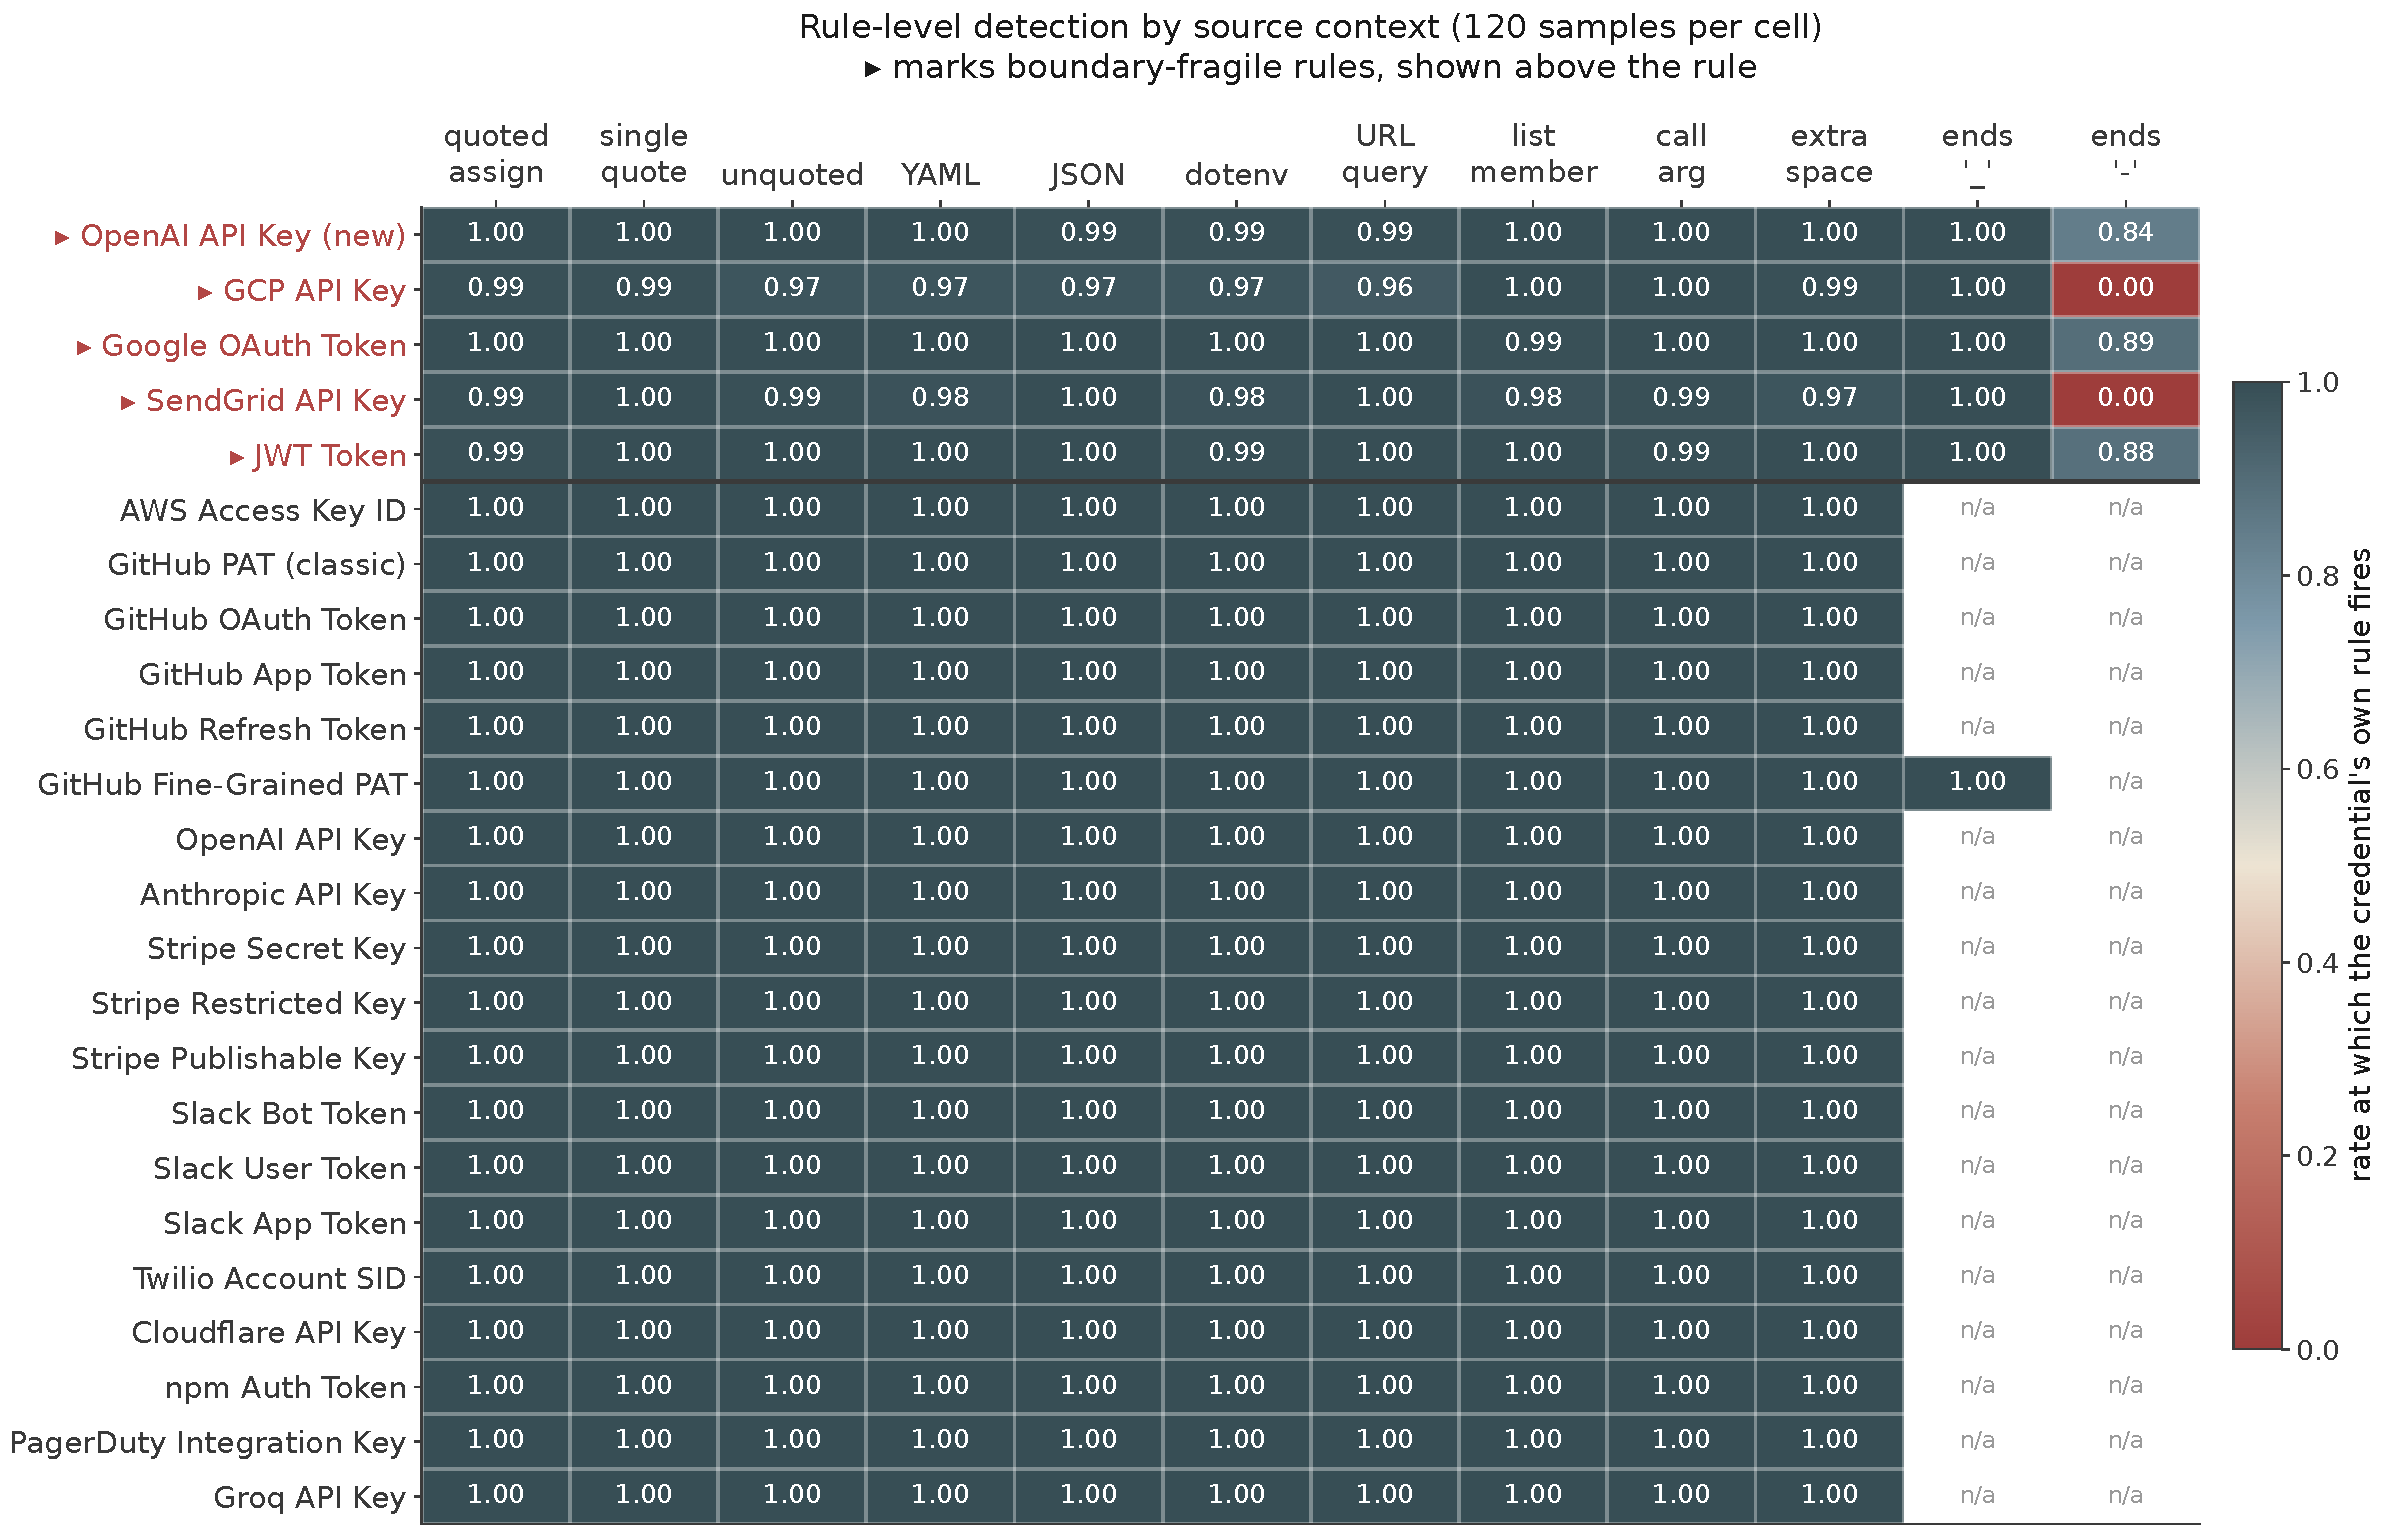
\includegraphics[width=\textwidth]{fig02_mutation_heatmap.pdf}
\caption{Rule-level detection across 24 rules and 12 contexts, 120 samples per cell. Blue indicates the credential's own rule fired; red indicates it did not. ``n/a'' marks embeddings not applicable to that rule. A leading $\blacktriangleright$ marks a boundary-fragile rule, listed above the robust rules and coloured red.}
\label{fig:heatmap}
\end{figure}

\section{RQ2: Mechanism and Marginal Probability}
\label{sec:rq2}

Five rules are boundary-fragile: \emph{OpenAI API Key (new)}, \emph{GCP API Key}, \emph{Google OAuth Token}, \emph{SendGrid API Key}, and \emph{JWT Token}.

\textbf{Mechanism 1: the anchor.} Each ends with \verb|\b| immediately after a character class containing a hyphen, e.g.
\begin{center}
\lstinline!r"\bSG\.[a-zA-Z0-9_-]{22}\.[a-zA-Z0-9_-]{43}\b"!
\end{center}
A hyphen is not a word character. When the final generated character is a hyphen and the following text character is also non-word --- a closing quote, in the canonical case --- no word boundary exists there and the match fails before any suppression logic runs. We confirmed that in failing samples every suppression predicate returns \texttt{False}: the scanner's own heuristics judge the value to be a credential, yet nothing is reported.

\textbf{Mechanism 2: quantifier type.} The failure is not uniform, and the split is exact (Fig.~\ref{fig:mechanism}a): fixed-count quantifiers admit no backtracking and fail totally, while variable-count quantifiers backtrack and match one character less.

\begin{center}\small
\begin{tabular}{@{}llr@{}}
\toprule
Rule & Quantifier & Rule fires \\
\midrule
SendGrid API Key & \texttt{\{43\}} fixed & 0.0\% \\
GCP API Key & \texttt{\{35\}} fixed & 0.0\% \\
OpenAI API Key (new) & \texttt{\{50,\}} variable & 84.2\% \\
JWT Token & \texttt{\{10,\}} variable & 88.3\% \\
Google OAuth Token & \texttt{\{68,\}} variable & 89.2\% \\
\botrule
\end{tabular}
\end{center}

The variable case is not benign: the rule reports a \emph{truncated} credential. We isolated this on a minimal pair --- \verb|\bX[a-zA-Z0-9_-]{10}\b| fails on a hyphen-terminated value while \verb|\bX[a-zA-Z0-9_-]{5,}\b| succeeds by matching one character fewer.

\textbf{Mechanism 3: why some failures are silent.} The entropy fallback captures candidates with \lstinline!['\"]([a-zA-Z0-9+/=_\-]{20,})['\"]!, a class excluding the dot. Credentials containing a dot (SendGrid, Google OAuth, JWT) cannot be rescued and become silent misses; dotless ones (GCP, OpenAI) are rescued but relabelled from \textsc{critical}/\textsc{high} to \textsc{medium} (Fig.~\ref{fig:fragile}). This is the distinction $RLP(\rho)$ and $SP(\rho)$ are defined to capture, and it is why GCP's preservation score is the lowest in Table~\ref{tab:metrics} despite its detection failures being the \emph{least} silent of the five.

\begin{figure}[t]
\centering
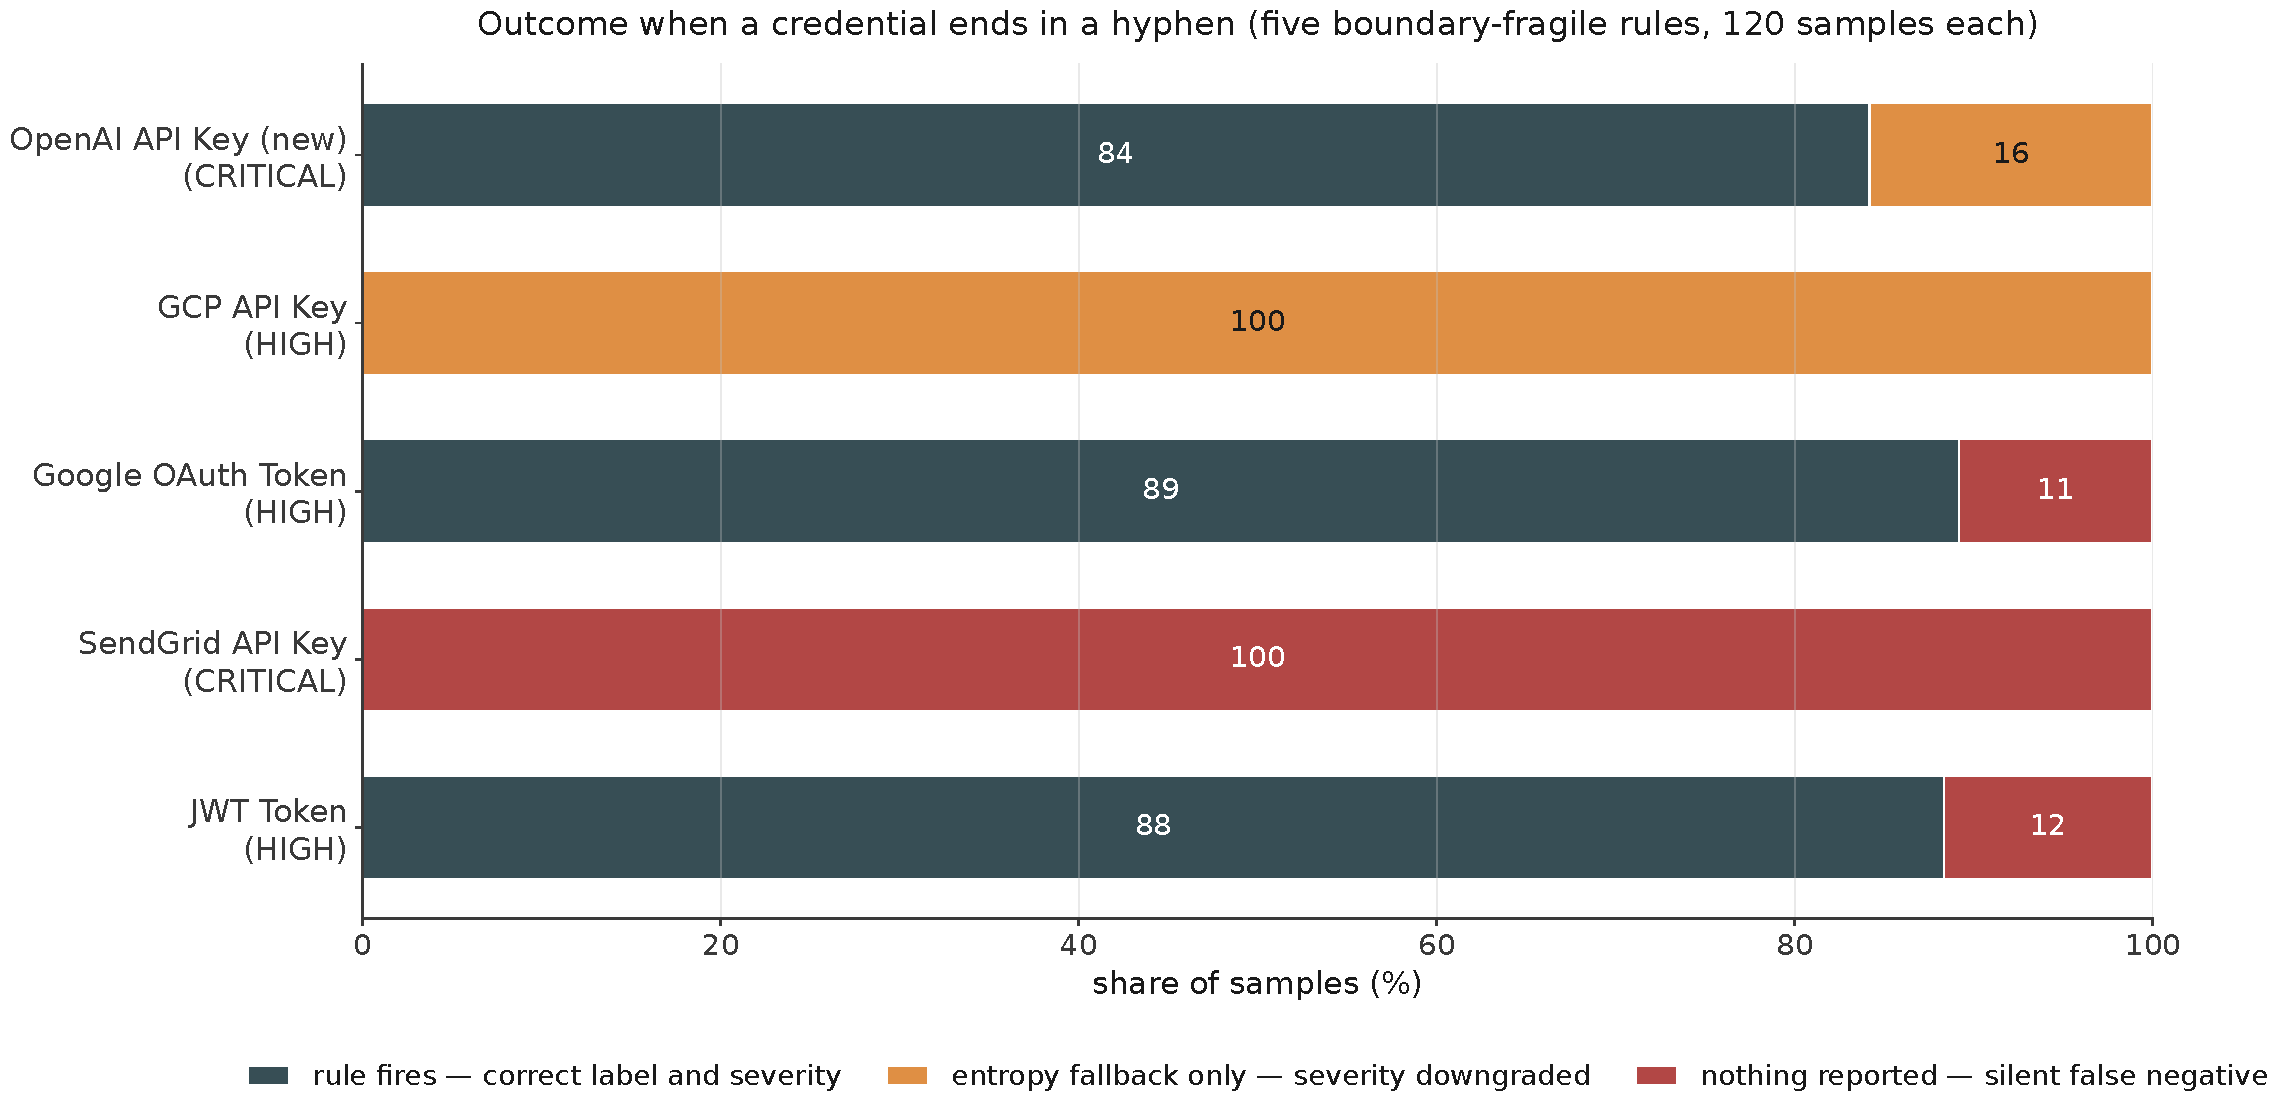
\includegraphics[width=0.98\textwidth]{fig03_fragile_outcomes.pdf}
\caption{Outcome decomposition for the five boundary-fragile rules when the credential ends in a hyphen. The two rules with $BR = 0$ fail in opposite ways: SendGrid is never reported at all, while GCP is always reported but always downgraded. A tool-level metric would score GCP and OpenAI as fully detected.}
\label{fig:fragile}
\end{figure}

\subsection{Marginal, not conditional, probability}

The rates above are \emph{conditional} on the credential ending in a hyphen. The marginal rate is
\[
P(\text{fail}) = P(\text{ends in ``-''}) \times P(\text{fail} \mid \text{ends in ``-''}),
\]
and $P(\text{ends in ``-''})$ is \emph{not} $1/64$ for every type. Two cases must be separated.

For types whose tail is a uniform draw over the 64-symbol base64url-style alphabet (SendGrid, GCP, OpenAI, Google OAuth), $P(\text{ends in ``-''}) = 1/64$ exactly, since the alphabet contains exactly one hyphen symbol and every symbol is equally likely; we report this exact value rather than a simulated one, and confirm it is not being misapplied with five independent $2\times10^5$-draw Monte Carlo checks from a cryptographic generator ($0.015555$--$0.015825$ across the five checks, consistent with $1/64 = 0.015625$ to within sampling error).

For JSON Web Tokens the tail is a base64url \emph{encoding} of a signature of $L$ bytes, and the final character carries only the residual bits: 6 bits when $L \equiv 0 \pmod 3$, 4 bits when $L \equiv 2$, and 2 bits when $L \equiv 1$. The character ``-'' has base64url index 62, which is not a multiple of 4 or 16, so it is reachable \emph{only} when $L \equiv 0 \pmod 3$. HS256 uses a 32-byte signature ($32 \bmod 3 = 2$), and we confirm empirically that only 16 distinct final characters occur and ``-'' never does. \textbf{An HS256 JWT is therefore structurally immune to this defect.} HS384 (48 bytes, $\equiv 0$) is not.

Table~\ref{tab:marginal} gives the corrected marginal rates. The practically consequential case is SendGrid, at exactly one credential in 64; the JWT case, which an earlier draft of this work overstated, is either impossible or roughly one in 548 depending on the signature algorithm.

\begin{table}[t]
\centering
\caption{Marginal probability that a credential is not correctly labelled}
\label{tab:marginal}
\small
\setlength{\tabcolsep}{3.5pt}
\begin{tabular}{@{}lrrl@{}}
\toprule
Credential type & $P(\text{``-''})$ & Marginal & Frequency \\
\midrule
SendGrid API Key & 1/64 & 0.015625 & 1 in 64 (silent miss) \\
GCP API Key & 1/64 & 0.015625 & 1 in 64 (downgraded) \\
Google OAuth Token & 1/64 & 0.001692 & 1 in 591 \\
JWT, HS384 (48 B) & 1/64 & 0.001823 & 1 in 548 \\
JWT, HS256 (32 B) & 0 & 0.000000 & impossible \\
\botrule
\end{tabular}
\end{table}

\begin{figure}[t]
\centering
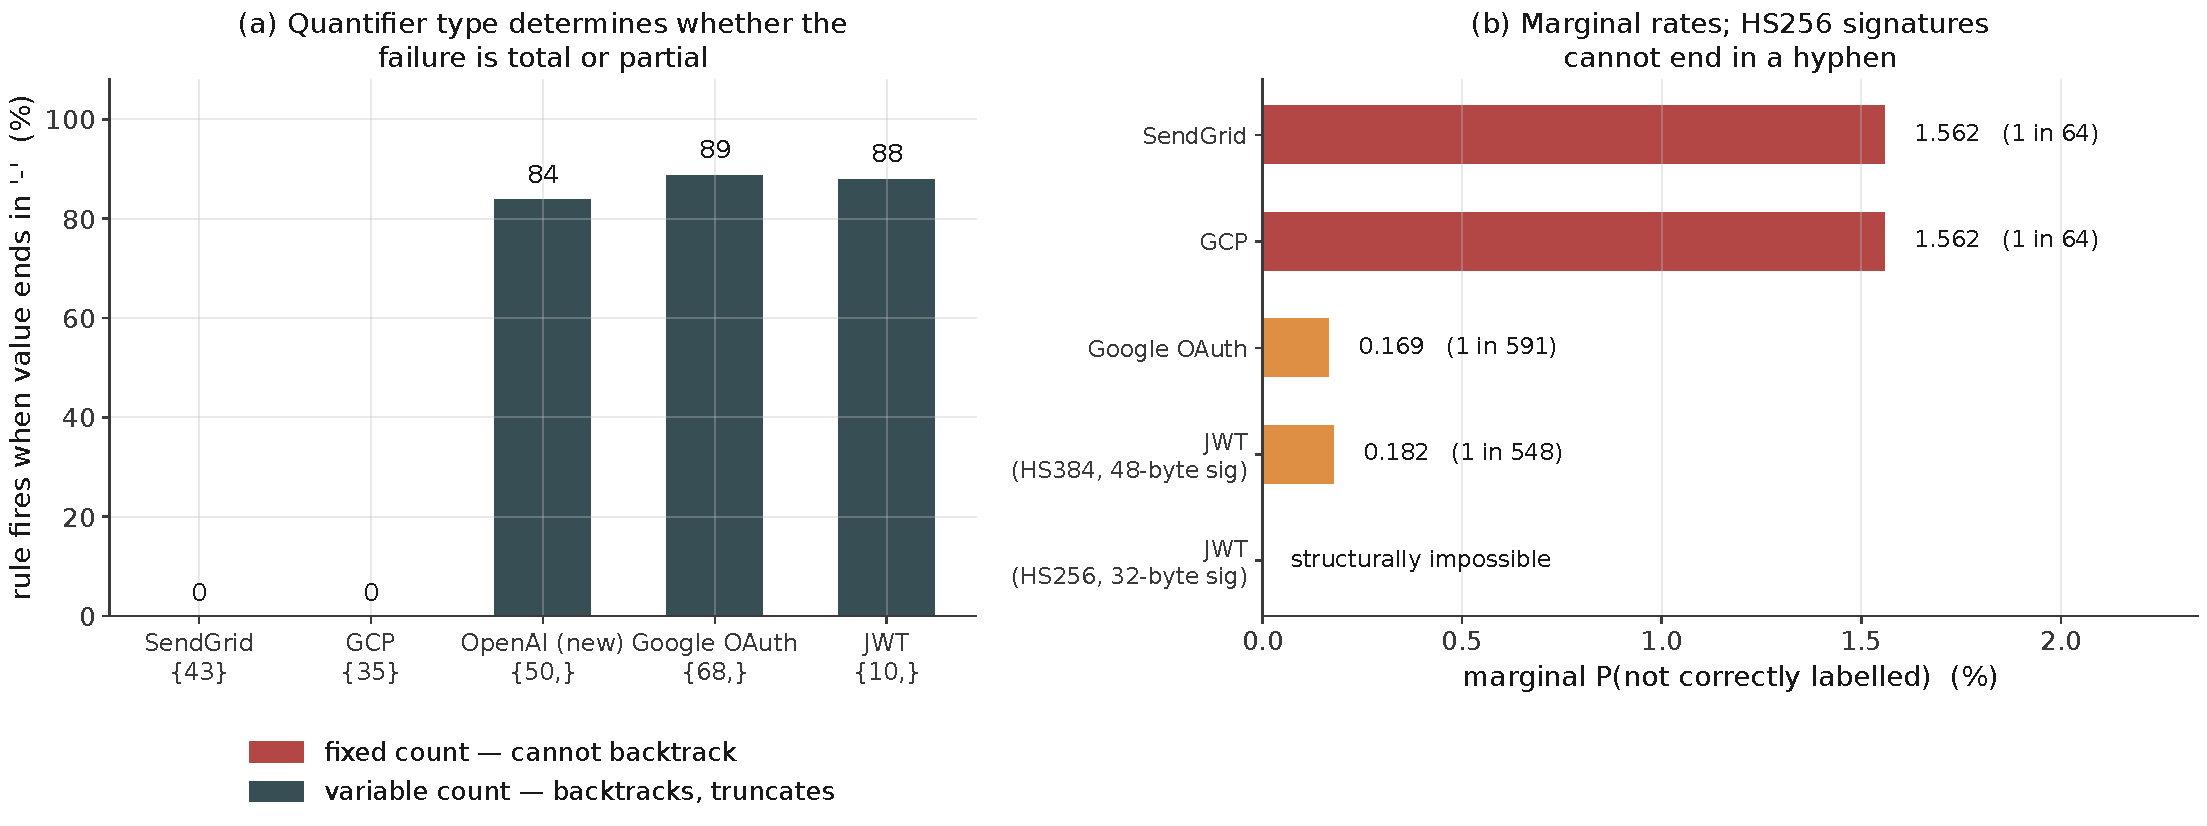
\includegraphics[width=0.94\textwidth]{fig04_mechanism.pdf}
\caption{(a) Quantifier type determines whether the failure is total or partial. (b) Corrected marginal rates; the encoding structure of HS256 signatures makes the defect unreachable for them.}
\label{fig:mechanism}
\end{figure}

The remedy is small and local: replace the trailing \verb|\b| with a negative lookahead, \verb+(?![A-Za-z0-9_])+, in the five affected rules. We do not merely propose this --- Section~\ref{sec:repair} applies it, re-runs the full battery, and reports a regression we found in a plausible first attempt at the same fix.

\section{Automated Repair and Fix Validation}
\label{sec:repair}

Diagnosing a defect and proposing a remedy is not evidence that the remedy works. This section applies two candidate repairs to the five affected rules, in memory, without modifying the subject repository, and re-runs the full boundary-mutation battery against each.

\subsection{Two candidates}

Both replace the trailing \verb|\b| that Section~\ref{sec:rq2} identifies as the fault:
\begin{itemize}
\item \textbf{Candidate A}, \verb+(?=[^\w-]|$)+, our first attempt: require the following character to be neither a word character nor a hyphen.
\item \textbf{Candidate B}, \verb+(?![A-Za-z0-9_])+, the recommended fix: require only that the following character is not a word character, which is what \verb|\b| itself requires and is the minimal change that removes the hyphen special case.
\end{itemize}
Both are applied to exactly the five rules of Table~\ref{tab:metrics}, holding every other rule and the entropy fallback unchanged.

\subsection{Both candidates repair the defect}

Fig.~\ref{fig:repair}a re-runs the full boundary-mutation battery under each candidate. Both restore $BR = 1.0$ on all five rules: the hyphen-terminated case that previously failed at $0$--$89\%$ now fires at $100\%$ under either fix. Neither candidate introduces a single new finding on the 292{,}527-line real-code corpus of Section~\ref{sec:rq5}: 67 findings under the baseline rule table, and 67 under each candidate, file for file.

\subsection{Candidate A regresses; Candidate B does not}
\label{sec:regression}

A repair to an anchoring assertion can fail in a direction the boundary battery does not by itself probe: it can become \emph{stricter} than the assertion it replaces, silently rejecting inputs the original correctly accepted. We therefore added one further probe, run under each candidate: a credential whose \emph{own} final character is an ordinary word character, immediately followed by a hyphen in the surrounding text (for example, a credential embedded as \verb|cfg_value = "...X-suffix"|). The original \verb|\b| accepts this case --- the boundary between a word character and a hyphen is a valid word boundary --- so a correct repair must continue to accept it.

Candidate A does not. Fig.~\ref{fig:repair}b shows it regressing to total failure ($0\%$) on exactly the two rules governed by fixed-count quantifiers, SendGrid and GCP, on precisely this case --- the same failure mode Section~\ref{sec:rq2} diagnosed, reintroduced by the fix. The cause is the same construct that caused the original defect: \verb+(?=[^\w-]|$)+ forbids a hyphen in the following text unconditionally, including here, where a hyphen legitimately follows a word-character-terminated credential. Candidate B imposes no such restriction and fires at $100\%$ on all five rules under this probe, matching the original rule's behaviour on the case it already handled correctly.

\begin{figure}[t]
\centering
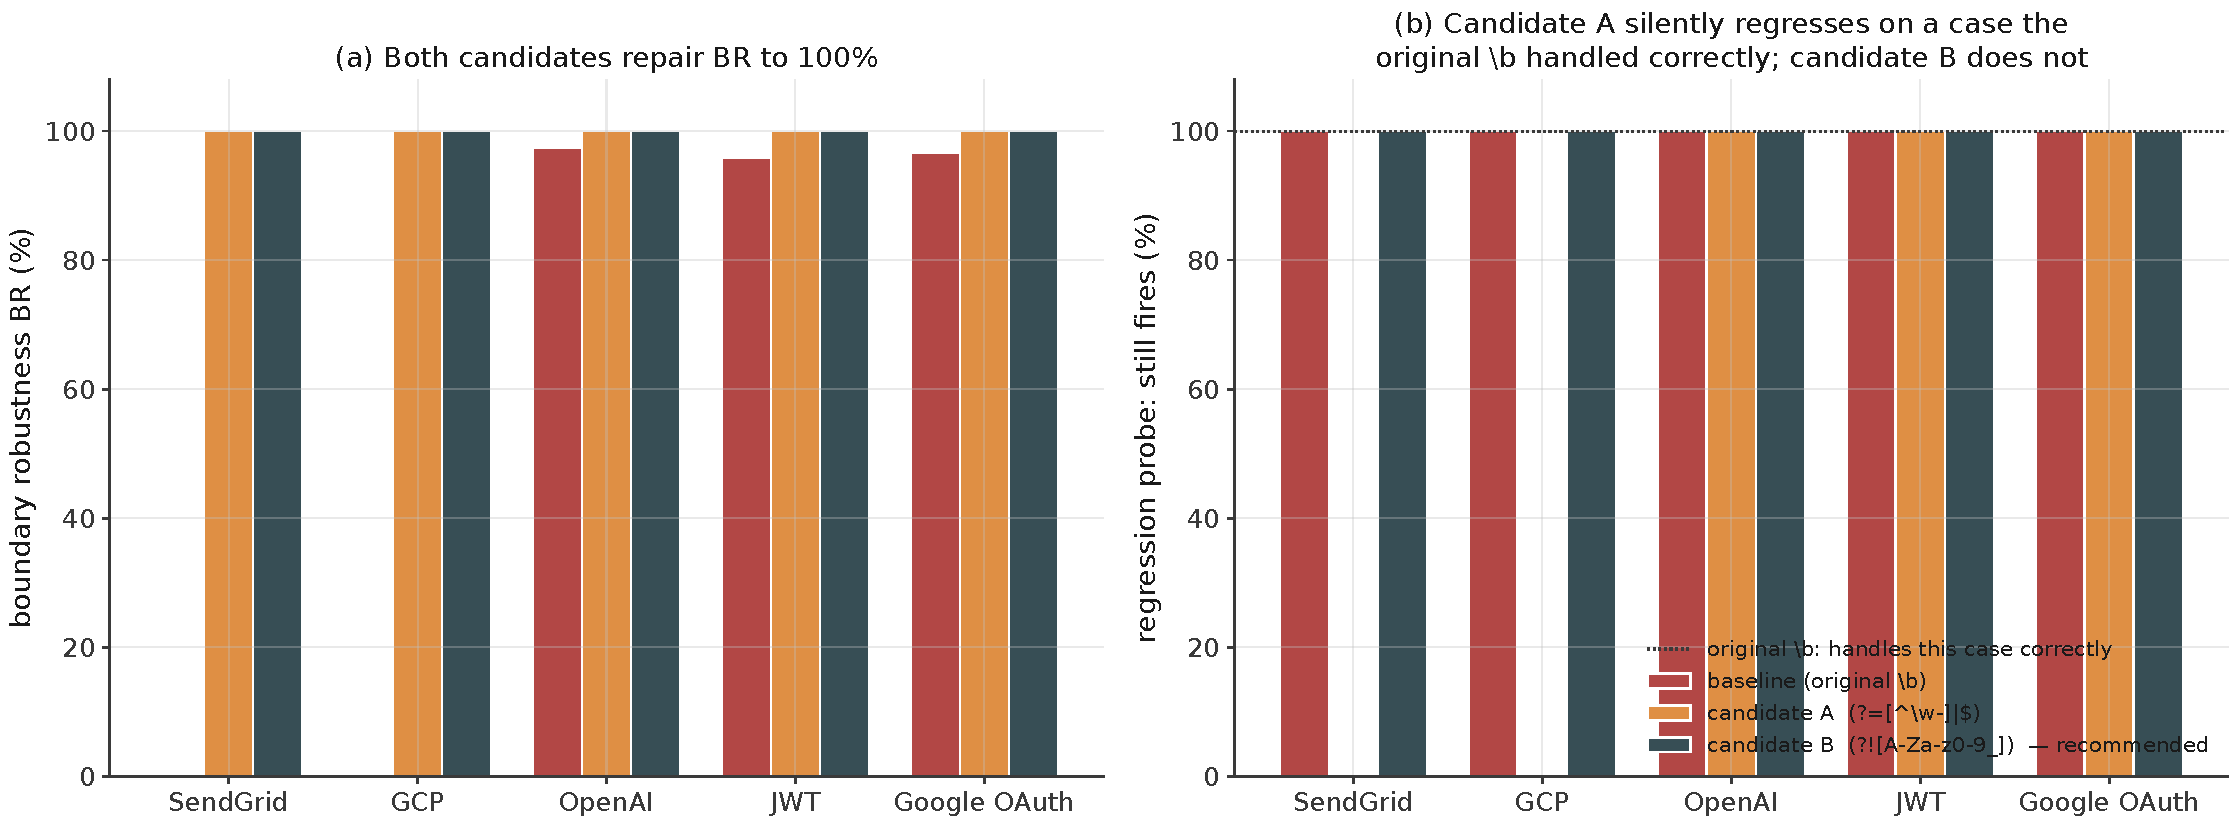
\includegraphics[width=0.94\textwidth]{fig04b_repair.pdf}
\caption{Fix validation. (a) Both candidates repair boundary robustness to $1.0$ on all five affected rules. (b) A regression probe --- a credential ending in a word character, followed by a hyphen --- that the original rule handled correctly. Candidate A silently fails it on the two fixed-count-quantifier rules; Candidate B does not.}
\label{fig:repair}
\end{figure}

This is the paper's second methodological point, not only its first result: a plausible one-line regex repair, chosen by inspection and applied to exactly the rules it was meant to fix, introduced a new defect of the same kind it removed. We found this only because we ran an oracle-based probe against the fix rather than reading it. We recommend Candidate B, \verb+(?![A-Za-z0-9_])+, and report both results because a method for finding hidden assumptions in a detection rule should be applied to its own proposed repair, not only to the original.

\section{RQ3: Does the Method Transfer?}
\label{sec:rq3}

We applied the identical battery to Gitleaks and TruffleHog, over 4{,}320 files. For external tools the expected rule per credential type is determined \emph{empirically} from each tool's own behaviour in the canonical context --- whichever \texttt{RuleID} or \texttt{DetectorName} it fires there --- so no tool is judged against another project's naming. Types a tool never fires on are excluded from its aggregate and reported separately, so coverage gaps are not scored as fragility.

\subsection{On ten shared types}

Fig.~\ref{fig:crosstool} shows the result on the ten types: \textbf{the method transfers, and exposes a distinct behavioural profile in each tool}. Two of the three degrade, and they degrade in different contexts; the third appears not to degrade at all. Section~\ref{sec:rq3-scale} shows that this last appearance does not survive scale.

\begin{figure}[t]
\centering
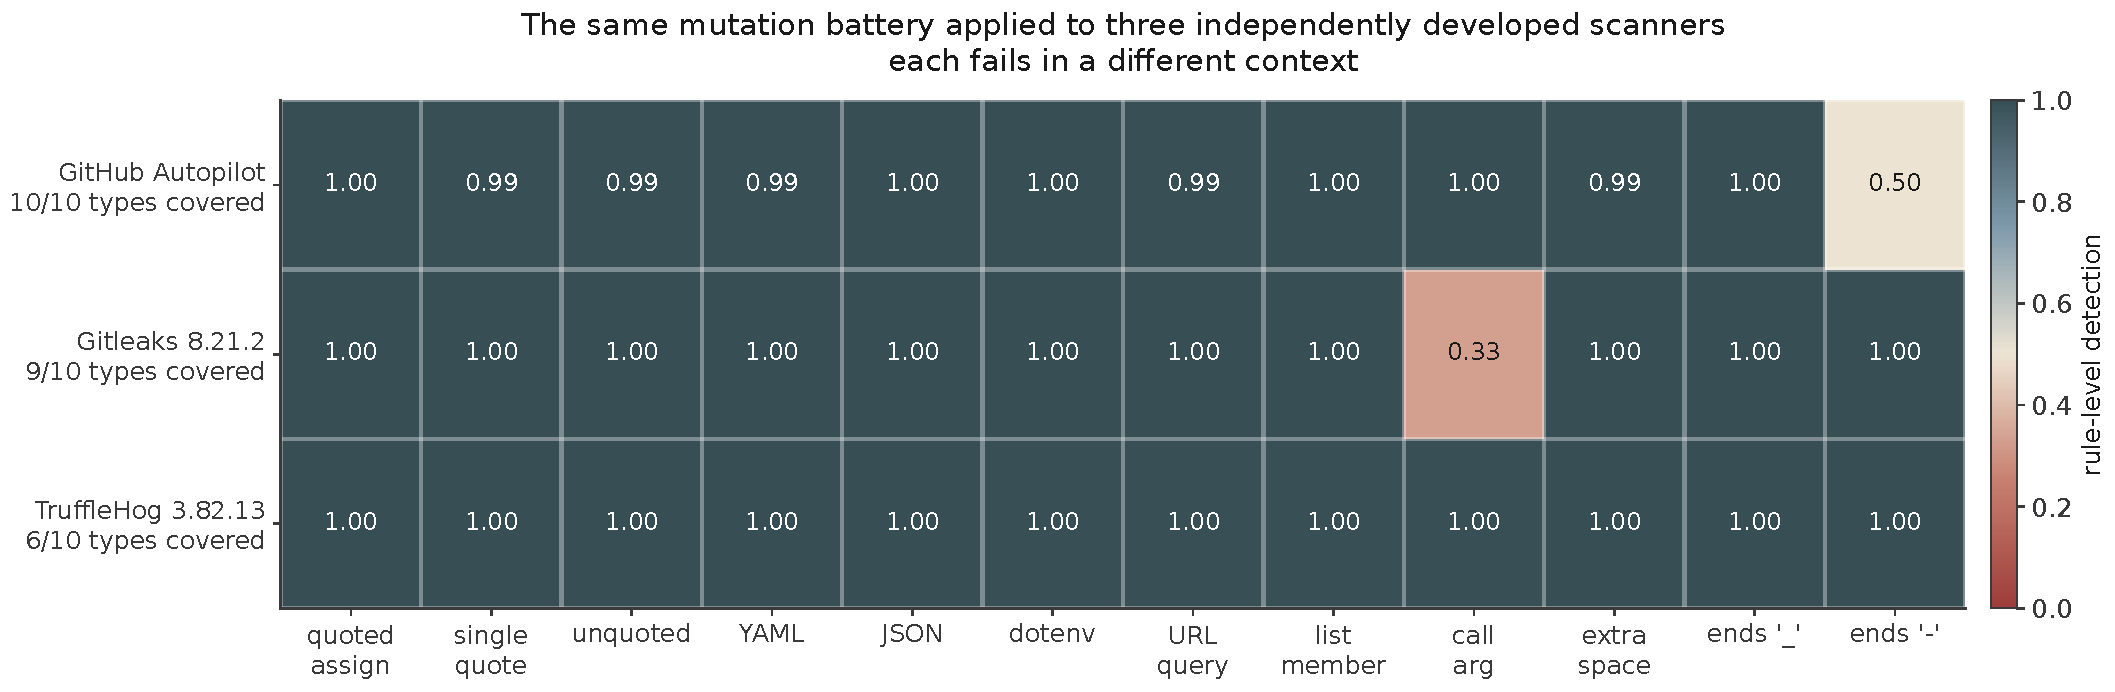
\includegraphics[width=0.94\textwidth]{fig05_crosstool.pdf}
\caption{The same mutation battery applied to three independently developed scanners. The battery reveals scanner-specific degradation patterns; no tested context degraded all three scanners.}
\label{fig:crosstool}
\end{figure}

\textbf{A second, unrelated defect in Gitleaks.} Gitleaks is unaffected by the trailing hyphen, but its rule-level detection falls to $0.333$ when a credential appears as a bare call argument. Per-type inspection of the nine shared credential types it detects shows this is not uniform: \texttt{github-pat}, \texttt{github-oauth} and \texttt{slack-bot-token} are unaffected, while \texttt{aws-access-token}, \texttt{gcp-api-key}, \texttt{npm-access-token}, \texttt{stripe-access-token}, \texttt{sendgrid-api-token} and \texttt{jwt} all drop to $0.000$ --- total misses.

To isolate the mechanism we ran a delimiter probe varying \emph{only} the single character following the credential (Fig.~\ref{fig:delim}). Gitleaks accepts end-of-line, both quote characters, whitespace, semicolon, backtick and colon, and rejects comma, closing parenthesis, closing bracket, closing brace, ampersand, forward slash, angle bracket and question mark. We confirmed the mechanism directly from source: Gitleaks' public configuration, \texttt{config/gitleaks.toml} at tag \texttt{v8.21.2}, defines each affected rule (\texttt{aws-access-token}, \texttt{gcp-api-key}, \texttt{npm-access-token}, \texttt{sendgrid-api-token}, \texttt{stripe-access-token}, \texttt{jwt}) with an identical trailing non-capturing group appended to the credential-capturing group, \lstinline!(?:['|\"|\n|\r|\s|\x60|;]|$)!, a Go regular-expression character class containing only the literal characters \texttt{'}, \texttt{|}, \texttt{"}, newline, carriage return, whitespace, backtick, and semicolon, or end-of-string. Every terminator we found rejected is provably absent from this class; every terminator we found accepted is provably present in it. The three unaffected types --- \texttt{github-pat}, \texttt{github-oauth}, \texttt{slack-bot-token} --- carry no such trailing group in their source regex at all, which is the source-level reason our data found them robust. We additionally verified the effect on minimal hand-written cases outside the harness: \texttt{cfg = "AKIA\ldots"} is detected, \texttt{f(AKIA\ldots)} is not.

The security relevance is direct. Every rejected character occurs routinely where credentials appear: \texttt{f(token)} in code, \texttt{[tok, x]} in a list, and --- most consequentially --- \texttt{?key=SECRET\&next=1} in a URL, which is among the more common shapes in which credentials actually leak.

\begin{figure}[t]
\centering
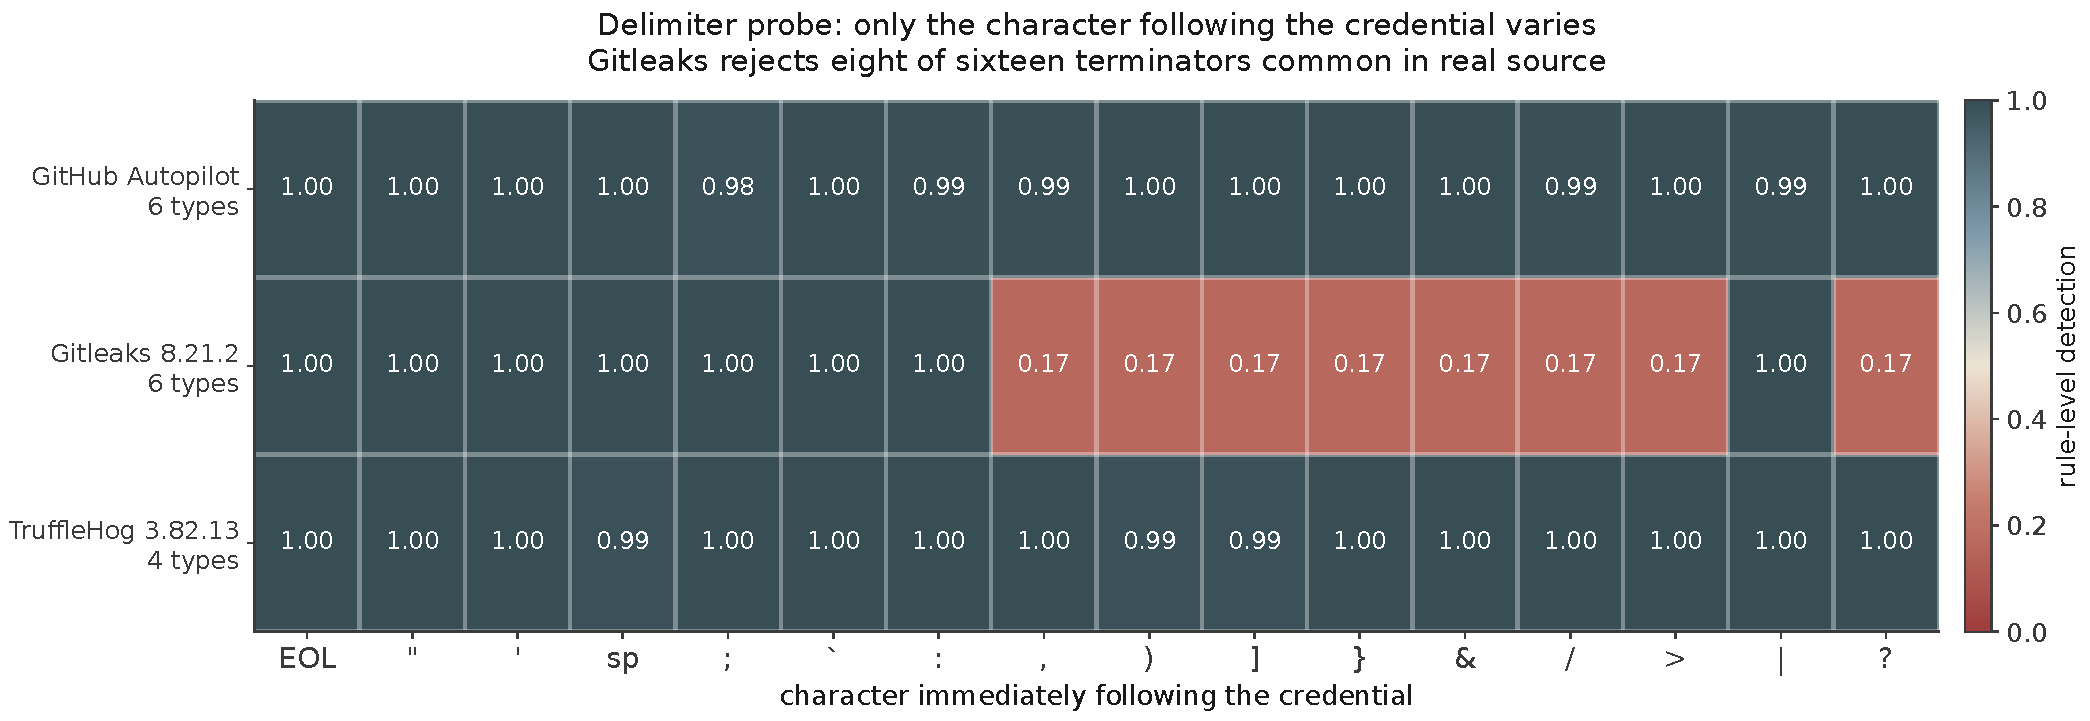
\includegraphics[width=0.94\textwidth]{fig06_delimiter.pdf}
\caption{Delimiter probe: only the character immediately following the credential varies. Gitleaks rejects eight of sixteen terminators that occur routinely in real source.}
\label{fig:delim}
\end{figure}

\textbf{TruffleHog appears robust on the ten types.} It is robust across every context and terminator on the six of ten types it covers canonically. Of those six, only one --- SendGrid --- has a format that permits a final hyphen, and TruffleHog's SendGrid pattern ends in a variable-count quantifier, \verb|[\w\-]{39,50}\b|, which backtracks to a match one character shorter exactly as Mechanism~2 of Section~\ref{sec:rq2} describes. The ten-type evidence for TruffleHog's boundary robustness is therefore one type, detected through a truncated match.

\subsection{At the scale of the full rule tables}
\label{sec:rq3-scale}

\textbf{Every Gitleaks rule.} A second harness runs the battery over every rule in Gitleaks' table, generating each credential from that rule's own secret group, so that the expected rule is the generating rule and no freezing is needed. Of 195 rules, 183 are analysed (88 identify the credential by its own prefix, 95 are keyword-anchored); 12 are excluded and listed: 3 apply only to particular file paths, and 9 yield fewer than 40 filter-valid samples in 400 draws from a neutral context (mostly structural rules for \texttt{curl} commands, webhook URLs and similar). A credential followed by `\texttt{)}' is missed entirely by 38 of the 88 prefix rules and all 95 keyword rules (Table~\ref{tab:fulltable}). Every one of those 133 rules carries the terminator group; of the 50 prefix rules without it, 49 pass. A minimal-pair control --- the same line with one space before `\texttt{)}' --- rescues 133 of the 134 failing rules; the exception, \texttt{huggingface-access-token}, also has a leading-character allowlist that excludes `\texttt{(}'. The association is total (two-sided Fisher exact test on the prefix rules, $p = 3.3\times10^{-24}$), but it was predicted from the configuration and is close to a restatement of it; the result the test adds is prevalence, not mechanism.

\begin{table}[t]
\centering
\caption{Gitleaks' full rule table: rules missing a credential followed by `\texttt{)}', by whether the rule carries the terminator group}
\label{tab:fulltable}
\small
\begin{tabular}{@{}lrrr@{}}
\toprule
Stratum & Rules & Terminator group & Miss on `\texttt{)}' \\
\midrule
Prefix, with group & \multirow{2}{*}{88} & 38 & 38 \\
Prefix, without group & & 50 & 1 \\
Keyword-anchored & 95 & 95 & 95 \\
\botrule
\end{tabular}
\end{table}

\textbf{A further Gitleaks defect.} Two rules, \texttt{huggingface-access-token} and \texttt{huggingface-organization-api-token}, miss every unquoted token in the unquoted, YAML and dotenv contexts. Both patterns end in a terminator class without the newline --- for the first, \verb!(?:$|[\\'"` <])! --- and Go's \verb|$| without the \texttt{(?m)} flag matches only at the very end of the text. A token followed by a line break --- any unquoted token not on the last line of its file --- is therefore missed. We confirmed this on four hand-written files outside the harness: the same token is detected without a trailing newline or in quotes, and missed with a newline or a following line. We have not found this defect reported.

\textbf{All three tools at 774 types.} Table~\ref{tab:battery774} gives, for each tool and the label-matched types it covers, how many types each context defeats entirely. Gitleaks' terminator defect generalises: `\texttt{)}' defeats 159 of its 218 types and `\texttt{\&}' in a query string 161. TruffleHog's apparent robustness does not: a trailing hyphen defeats 91 of the 117 types whose own format allows one. The mechanism is the primary subject's. Of the 91 failing types, 88 were generated from TruffleHog's own detectors, and all 88 of those detectors' patterns end in \verb|\b|, for instance \verb|\b(glpat-[a-zA-Z0-9\-=_]{20,22})\b|, and a fixed or exhausted minimum length leaves no room to backtrack. We confirmed it on minimal pairs outside the harness for the GitLab and Apify detectors: a hyphen-terminated token is missed quoted, unquoted, and followed by a space. In the primary subject, 4 of its 39 label-matched types fail every non-canonical context, including the spaced controls; these are keyword-anchored rules that require a quoted value, a narrower defect than a boundary one.

\begin{table}[t]
\centering
\caption{Types missed entirely, of the label-matched types each tool covers. The trailing-comma context is a quoted list element for self-identifying types and a keyword argument followed by a comma for keyword-anchored ones. The spaced control adds one space before `\texttt{)}'.}
\label{tab:battery774}
\small
\setlength{\tabcolsep}{5pt}
\begin{tabular}{@{}lrrr@{}}
\toprule
Context & Primary subject & Gitleaks & TruffleHog \\
\midrule
types covered (label-matched) & 39 & 218 & 580 \\
\midrule
unquoted & 4 & 2 & 0 \\
trailing comma & 4 & 108 & 1 \\
call argument, `\texttt{)}' & 4 & 159 & 1 \\
query string, `\texttt{\&}' & 4 & 161 & 1 \\
spaced control, `\texttt{\ )}' & 4 & 1 & 1 \\
\midrule
trailing hyphen (applicable types) & 3 / 8 & 1 / 65 & 91 / 117 \\
\botrule
\end{tabular}
\end{table}

\textbf{Marginal probabilities at scale.} For every type whose format allows a final hyphen, $P(\text{ends in ``-''})$ is estimated from 1{,}000 fresh draws of the type's own generator, under the uniform model of Section~\ref{sec:rq2}, and multiplied by each tool's conditional failure rate. For TruffleHog 86 of the 117 types reach a marginal failure probability of at least 1 in 100 (maximum 0.061); for the primary subject 3 of 8 (maximum 0.014, against the exact 1/64 of Table~\ref{tab:marginal} for SendGrid); for Gitleaks 1 of 65. These are estimates of the share of \emph{generated} credentials affected; Section~\ref{sec:rq6} turns to real code.

\textbf{Taxonomy.} At scale, two boundary-handling strategies account for every boundary defect we found. An \emph{implicit} anchor (\verb|\b|), used by the primary subject and by TruffleHog, fails as a function of the credential's own final character. An \emph{explicit} terminator allowlist, used by Gitleaks --- and in a variant with \verb|$| by its two Hugging Face rules --- fails as a function of the character that follows. The third profile seen at ten types, boundary independence, was an artefact of which types happened to be shared. The defect class is tool-specific; the vulnerability to boundary assumptions is not, and it reaches all three tools.

\section{RQ4: Comparison, Corpus, Deployment Condition, and Scale}
\label{sec:rq4}

\begin{table}[t]
\centering
\caption{Three scanners on identical corpora (400 positives, 700 negatives), with Wilson 95\% intervals. No value is emphasised: Section~\ref{sec:paired} shows that none of the between-tool differences is statistically significant at the correct unit of analysis.}
\label{tab:comparative}
\footnotesize
\setlength{\tabcolsep}{3pt}
\begin{tabular}{@{}llllll@{}}
\toprule
Corpus & Tool & Precision [95\% CI] & Recall [95\% CI] & F1 & TP / FP / FN \\
\midrule
\multirow{3}{*}{A: format-spec}
 & GitHub Autopilot & 0.959 [0.936, 0.974] & 1.000 [0.991, 1.000] & 0.979 & 400 / 17 / 0 \\
 & Gitleaks 8.21.2 & 1.000 [0.988, 1.000] & 0.800 [0.758, 0.836] & 0.889 & 320 / 0 / 80 \\
 & TruffleHog 3.82.13 & 1.000 [0.984, 1.000] & 0.598 [0.549, 0.644] & 0.748 & 239 / 0 / 161 \\
\midrule
\multirow{3}{*}{B: structural}
 & GitHub Autopilot & 0.959 [0.935, 0.974] & 0.998 [0.986, 1.000] & 0.978 & 399 / 17 / 1 \\
 & Gitleaks 8.21.2 & 1.000 [0.989, 1.000] & 0.900 [0.867, 0.926] & 0.947 & 360 / 0 / 40 \\
 & TruffleHog 3.82.13 & 1.000 [0.984, 1.000] & 0.600 [0.551, 0.647] & 0.750 & 240 / 0 / 160 \\
\botrule
\end{tabular}
\end{table}

Corpus construction alone moves Gitleaks' recall from $0.800$ to $0.900$: its JWT rule validates internal token structure and correctly refuses a ``JWT'' whose segments are random characters. The subject's scanner is almost unmoved, $1.000$ to $0.998$ --- not because it is more capable, but because its rules are shallower (prefix, class, length). That shallowness also produces its 17 false positives where the others have none.

\subsection{At ten types the comparison supports no ranking}
\label{sec:paired}

The intervals in Table~\ref{tab:comparative} are computed over samples, and taken at face value they do not overlap. That would be the wrong conclusion to draw, for a reason visible in the raw data: \emph{per-type detection is very nearly deterministic}. Across both corpora and all three tools, fifty-eight of the sixty per-type recall values are exactly $0.000$ or exactly $1.000$. The two exceptions are both $0.975$, a single miss in forty: TruffleHog on Slack bot tokens in corpus~A, and the subject on SendGrid keys in corpus~B. A tool either detects a credential type or it does not, with these two borderline exceptions; the 40 samples within a type are very close to 40 repetitions of one outcome rather than 40 independent observations.

We state this as a measured property rather than an assumption because we tested it. An earlier version of the comparative harness recorded a fixed seed in its output while drawing every credential from \texttt{secrets}, a CSPRNG that cannot be seeded; the corpus therefore differed on every run. Under one such draw all sixty values were exactly $0.000$ or $1.000$, which would have made the determinism premise look exact when it is not. With the seed actually applied and the corpus fixed, two cells sit at $0.975$. The inflation argument below is unaffected --- a factor of forty is not recovered by two samples --- but the premise is near-determinism, not determinism, and we report it as such.

The effective unit of analysis is therefore the credential \emph{type}, of which there are ten, and a sample-level test would overstate the evidence by a factor of 40. We accordingly compare tools with an exact paired sign test over the ten types, reporting the discordant types themselves rather than a test statistic alone (Table~\ref{tab:paired}).

\begin{table}[t]
\centering
\caption{Exact paired sign test over $n{=}10$ credential types. ``Discordant'' counts types detected by the first tool and not the second, and conversely.}
\label{tab:paired}
\small
\setlength{\tabcolsep}{4pt}
\begin{tabular}{@{}llrr@{}}
\toprule
Corpus & Comparison & Discordant & $p$ \\
\midrule
\multirow{3}{*}{A}
 & Autopilot vs.\ Gitleaks & 2 / 0 & 0.500 \\
 & Autopilot vs.\ TruffleHog & 4 / 0 & 0.125 \\
 & Gitleaks vs.\ TruffleHog & 2 / 0 & 0.500 \\
\midrule
\multirow{3}{*}{B}
 & Autopilot vs.\ Gitleaks & 1 / 0 & 1.000 \\
 & Autopilot vs.\ TruffleHog & 4 / 0 & 0.125 \\
 & Gitleaks vs.\ TruffleHog & 3 / 0 & 0.250 \\
\botrule
\end{tabular}
\end{table}

\textbf{No comparison reaches significance at $\alpha=0.05$}, and none comes close. The differences are entirely one-directional --- every discordant type favours the same tool, never the reverse --- which looks like a real ordering, but with ten types the sign test cannot resolve one: even a perfect $4/0$ split has $p = 0.125$, because $2^{-4}$ doubled is the smallest two-sided $p$-value ten paired types can produce at that margin. The design is underpowered for ranking by construction, and no larger sample of \emph{credentials} would fix it; only more credential \emph{types} would.

We therefore report Table~\ref{tab:comparative} as a characterisation of where the tools differ and why, and we draw no ranking from it. This bears directly on the competing interest declared in Section~\ref{sec:bias}: the raw numbers favour the author's own tool, and the correct statistical treatment does not support that advantage. The next subsection shows that withholding the ranking was right for a further reason: at scale, with the generator controlled, the ordering reverses.

\subsection{At 774 types, with generator bias controlled}
\label{sec:rq4-scale}

Table~\ref{tab:coverage} counts, for each tool, the label-matched types it covers among those each generator produced. Generator bias is plain in it: each tool covers nearly every type its own rules generate (Gitleaks 183 of 184, TruffleHog 532 of 566, the primary subject 24 of 24), so any pooled comparison is weighted towards the tool that contributed most types. The ten-type corpora of Section~\ref{sec:paired} were built from published prefix, alphabet and length specifications --- the same shallow shape the primary subject's rules encode, which the first paragraph of this section already identified as the source of its apparent recall advantage --- and no generator from the other tools' rule tables was used.

\begin{table}[t]
\centering
\caption{Label-matched types covered, by the tool whose rules generated them}
\label{tab:coverage}
\small
\begin{tabular}{@{}lrrrr@{}}
\toprule
Covered by $\downarrow$ / generated by $\rightarrow$ & Gitleaks & TruffleHog & Primary subject & Total \\
 & (184) & (566) & (24) & (774) \\
\midrule
Primary subject & 9 & 6 & 24 & 39 \\
Gitleaks & 183 & 22 & 13 & 218 \\
TruffleHog & 37 & 532 & 11 & 580 \\
\botrule
\end{tabular}
\end{table}

The neutral comparison removes it: each pair is compared only on the types the third tool generated (Table~\ref{tab:neutral}). On TruffleHog's 566 types, Gitleaks covers 18 that the primary subject does not, and the subject 2 that Gitleaks does not ($p = 0.0004$, exact sign test). On Gitleaks' 184 types, TruffleHog covers 30 that the subject does not, and the subject 2 ($p = 2.5\times10^{-7}$). On the subject's 24 types, Gitleaks and TruffleHog differ by 3 to 1 ($p = 0.625$): no conclusion. Both comparisons that can be resolved place the primary subject last.

\begin{table}[t]
\centering
\caption{Neutral comparison: each pair of tools on the types generated by the third. ``Only'' counts label-matched types covered by one tool of the pair and not the other.}
\label{tab:neutral}
\small
\setlength{\tabcolsep}{3pt}
\begin{tabular}{@{}llrrrr@{}}
\toprule
Pair & Types from & $n$ & Only first & Only second & $p$ \\
\midrule
Primary subject vs.\ Gitleaks & TruffleHog & 566 & 2 & 18 & 0.0004 \\
Primary subject vs.\ TruffleHog & Gitleaks & 184 & 2 & 30 & $2.5\times10^{-7}$ \\
Gitleaks vs.\ TruffleHog & Primary subject & 24 & 3 & 1 & 0.625 \\
\botrule
\end{tabular}
\end{table}

\textbf{Mislabelling.} Without label matching the primary subject would appear to cover 132 types rather than 39. Of the 93 others, it reports 84 under its PagerDuty rule, which at the pinned commit is \verb|\b[a-z0-9]{32}\b| --- any 32-character lowercase word --- with no keyword; 8 under its generic JWT rule; and one under a generic token rule. Gitleaks mislabels 2 types, as generic JWTs; TruffleHog none. This is the rule-level oracle's second use: a tool-level oracle would have credited the subject with detecting 84 other providers' credentials, under a label and severity that are wrong for every one of them.

What this changes, and what it does not, should be explicit. The ten-type null result was a correct statement about ten types. The raw ordering it declined to report would have been wrong: the ordering that survives a neutral choice of generator runs the other way. Coverage is not the whole of quality --- the next paragraph shows that one tool's coverage depends on its deployment condition, and Section~\ref{sec:rq5} measures false positives --- but on the question this section can answer, the primary subject is the weakest of the three.

\textbf{Deployment condition matters more.} Our single-credential-per-file design is adversarial to co-occurrence-based detection, so we evaluated four conditions (Fig.~\ref{fig:cooc}): (A) a credential alone; (B) paired with its companion secret; (C) several credentials in one file; (D) a realistic settings module with imports, comments and unrelated configuration.

TruffleHog's detection rises from $0.667$ (A) to $0.833$ (B) to $1.000$ (C), settling at $0.828$ in the realistic condition (D). Per type, AWS goes from $0.000$ in isolation to $1.000$ once a secret access key accompanies it. Its apparent recall deficit in Table~\ref{tab:comparative} is therefore \textbf{substantially an artefact of the corpus}, not a capability limit, and the single-credential numbers should be read as a lower bound under conditions adversarial to that architecture. The other two tools are near-invariant across conditions.

\begin{figure}[t]
\centering
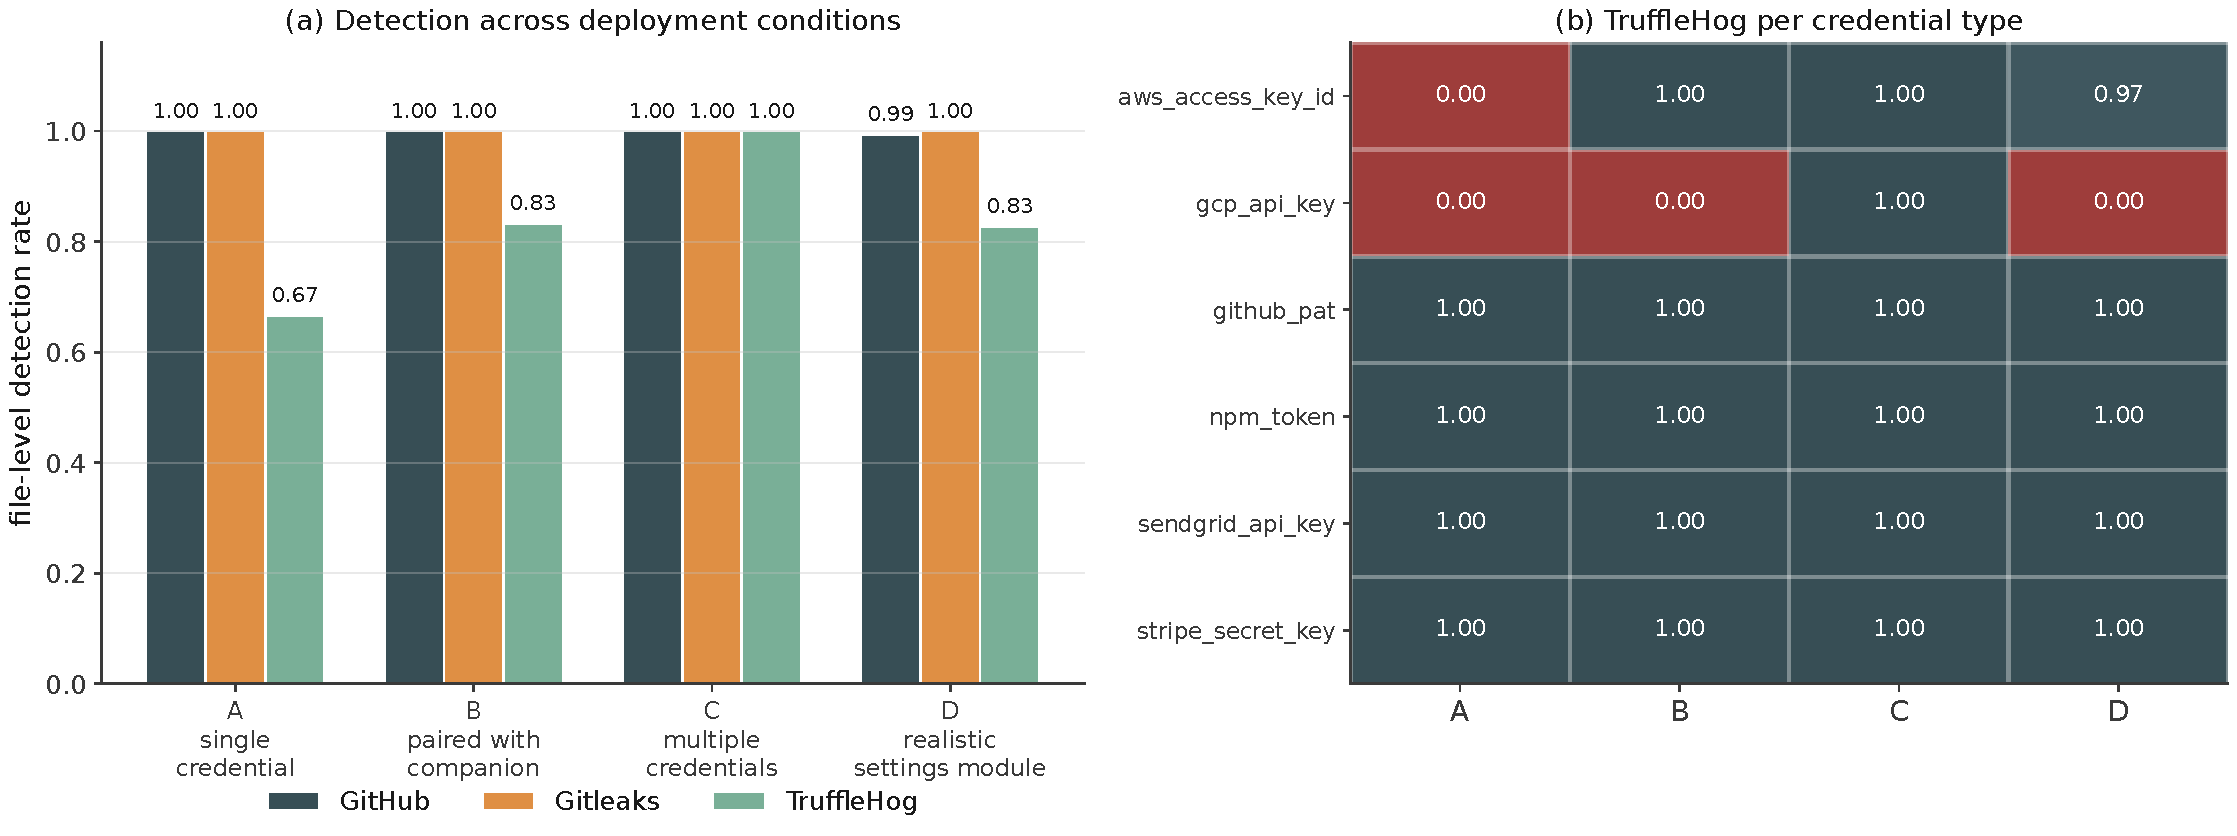
\includegraphics[width=0.94\textwidth]{fig07_cooccurrence.pdf}
\caption{Detection across four deployment conditions. TruffleHog's recall depends strongly on corroborating context; the other two tools do not.}
\label{fig:cooc}
\end{figure}

\section{RQ5: False Positives on Unmodified Real Code}
\label{sec:rq5}

\subsection{Four Python projects}

We scanned 292{,}527 lines of unmodified source from four open-source projects --- \texttt{requests}, \texttt{flask}, \texttt{redis-py}, and the subject --- line by line as added diff lines, mirroring the subject's push handler. All four are pinned by commit in the replication package.

This corpus is small and Python-centric, and it is not a sample of anything. We therefore make no claim about real-world false-positive rates in general; the claim is about \emph{these four projects}, and its purpose is to test whether a conclusion drawn from the synthetic corpus survives contact with unmodified code. It does not.

The ordering \emph{inverts} relative to the synthetic corpus (Fig.~\ref{fig:rw}). On constructed negatives the subject's scanner had the worst precision; on this corpus it has the lowest rate: $0.034$ findings per kLOC against Gitleaks' $0.208$ and TruffleHog's $0.233$. The synthetic corpus over-represented bare high-entropy base64 assignments, to which its unanchored fallback is uniquely vulnerable, and under-represented the documentation and configuration idioms that dominate real repositories.

We inspected all ten of its findings; every one is a false positive, in three groups: six occurrences of a documentation URL \emph{template} (\texttt{redis://[[username]:\allowbreak[password]]\allowbreak @localhost:6379/0}) matched at \textsc{critical} severity; three doctest passwords; and one RFC 3986 unreserved-character constant matched by the entropy fallback.

For fairness: 49 of Gitleaks' and 41 of TruffleHog's findings occur in the subject's own repository, which contains credential-shaped strings in its rule table and fixtures and which its scanner suppresses via path rules tuned for that layout. Restricted to the three third-party projects the totals are 10, 12, and 27.

These figures have a defect of their own, which the extended study exposed: the primary subject was given an extension allow-list of file types while Gitleaks and TruffleHog scanned every file, so the three tools did not see an identical file set. Re-scanned on one staged file set (next subsection), the same three projects at the same commits give 12, 12 and 27; only the subject's count changes. The ordering on these projects survives, but the corpus is too small to carry it, and the nine-language corpus does not reproduce it.

\begin{figure}[t]
\centering
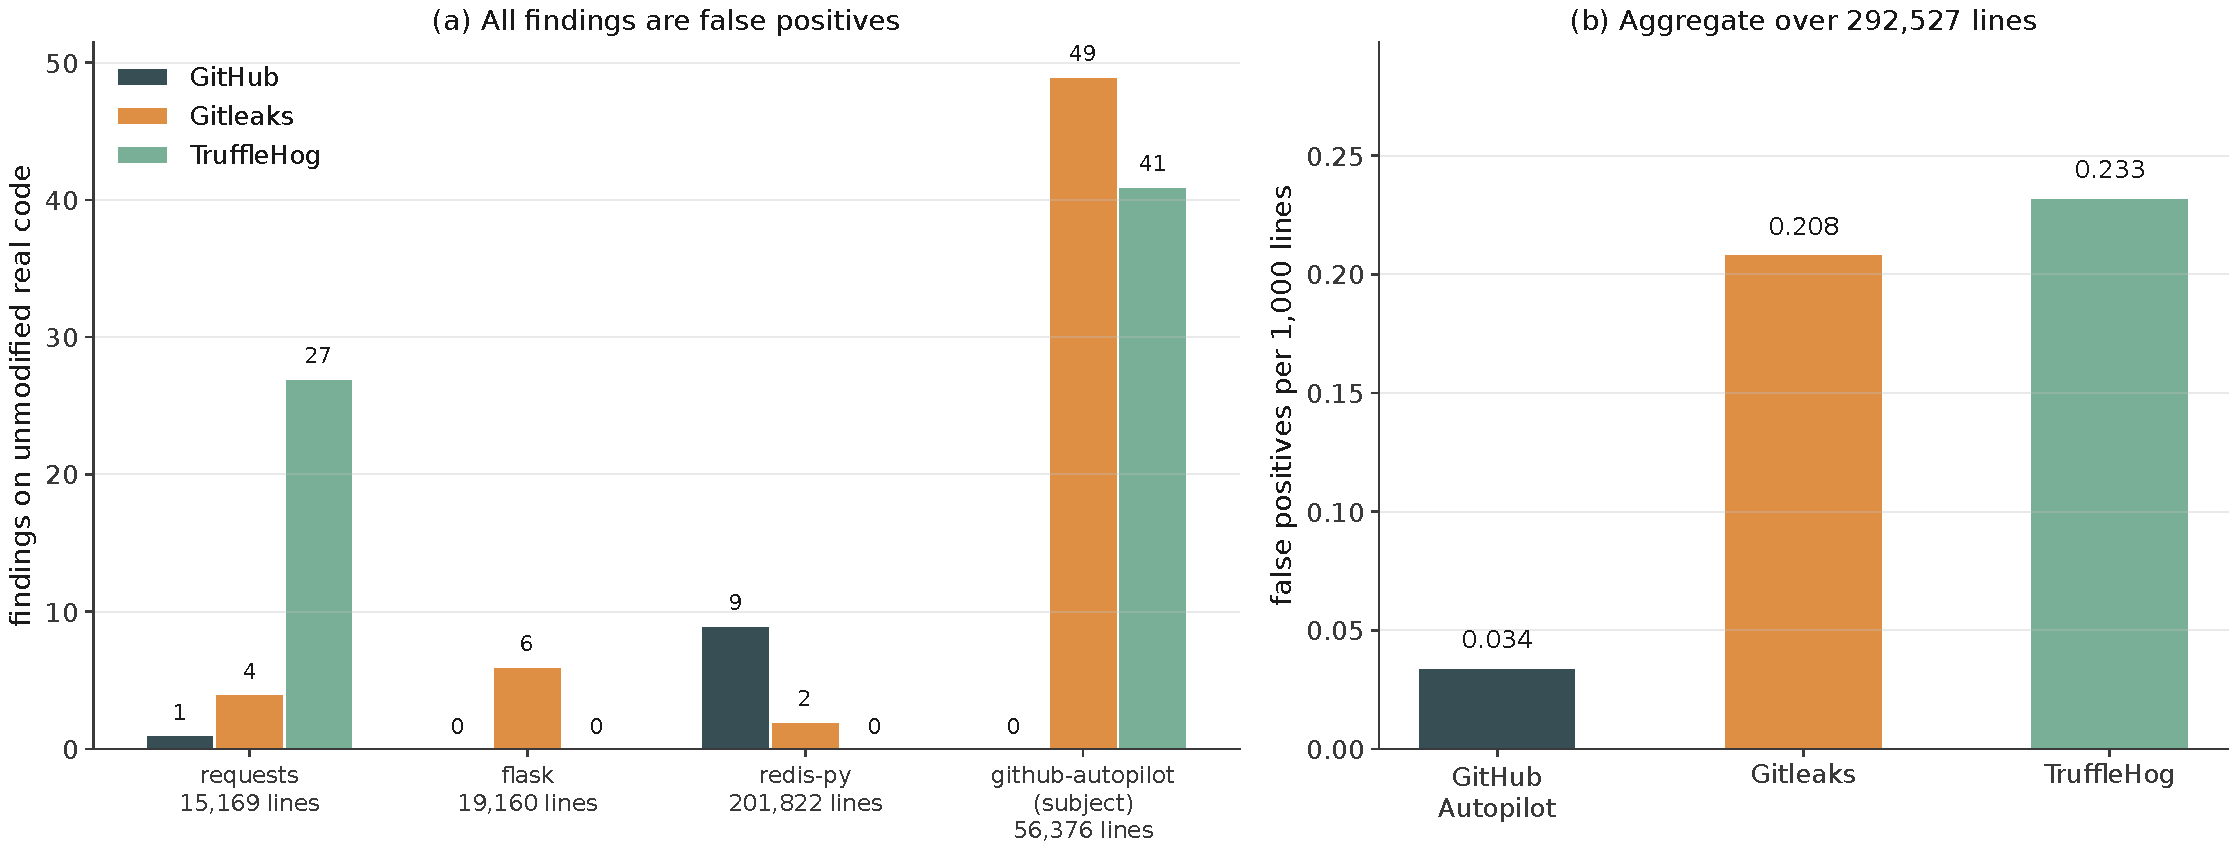
\includegraphics[width=0.94\textwidth]{fig08_realworld.pdf}
\caption{False positives on the four unmodified open-source projects evaluated. The ordering inverts relative to the synthetic corpus.}
\label{fig:rw}
\end{figure}

\subsection{Nine languages, one file set}

On the multi-language corpus every tool scans the same 38{,}309 files. Table~\ref{tab:fplang} gives findings per kLOC by language. Over all 9.87 million lines the primary subject reports 2{,}108 findings (0.214 per kLOC), Gitleaks 1{,}143 (0.116) and TruffleHog 389 (0.039); in the general stratum alone, 0.108, 0.036 and 0.038. The ordering on the four Python projects does not hold: on this corpus the primary subject has the highest rate overall, in the general stratum, and in six of the nine languages; TruffleHog's is highest in Go, JavaScript and PHP.

\begin{table}[t]
\centering
\caption{Findings per kLOC on 31 repositories, by language, on one staged file set}
\label{tab:fplang}
\small
\setlength{\tabcolsep}{3pt}
\begin{tabular}{@{}lrrrrr@{}}
\toprule
Language & Repositories & kLOC & Primary subject & Gitleaks & TruffleHog \\
\midrule
C\# & 2 & 387 & 0.028 & 0.003 & 0.000 \\
Go & 4 & 518 & 0.058 & 0.126 & 0.268 \\
Java & 3 & 997 & 0.024 & 0.003 & 0.000 \\
JavaScript & 3 & 3{,}916 & 0.011 & 0.008 & 0.013 \\
PHP & 2 & 589 & 0.087 & 0.053 & 0.110 \\
Python & 8 & 1{,}444 & 0.189 & 0.068 & 0.071 \\
Ruby & 3 & 649 & 0.014 & 0.006 & 0.006 \\
Rust & 2 & 143 & 0.084 & 0.056 & 0.056 \\
TypeScript & 4 & 1{,}227 & 1.347 & 0.735 & 0.016 \\
\midrule
All & 31 & 9{,}871 & 0.214 & 0.116 & 0.039 \\
\botrule
\end{tabular}
\end{table}

No finding is asserted to be a live credential; released public code is assumed to contain none. Findings are sorted by stated rules into placeholder or test values, findings under test, documentation or example paths, hash or identifier contexts, and the rest. The subject's 2{,}108 findings divide 1{,}406 / 177 / 4 / 521, Gitleaks' 1{,}143 divide 843 / 279 / 2 / 19, and TruffleHog's 389 divide 89 / 280 / 1 / 19. One repository, \texttt{Shopify/shopify-app-js}, contributes 1{,}530 of the subject's and 859 of Gitleaks' findings, almost all placeholder lines in test fixtures, which is why TypeScript dominates the table; without that repository the subject's rate is still the highest, though Gitleaks and TruffleHog change places. TruffleHog is the one tool whose output varied between runs on identical input (Section~\ref{sec:setup}); 2 findings were unstable and are not counted.

Literals in real code that carry a known provider prefix are scarce: 80 occurrences of 10 types in 9.87 million lines, 77 of them under test, documentation or example paths. Detection rates on them are reported in the replication package; they are too few to rank tools, and they are mostly in the paths the primary subject suppresses by design.

\section{RQ6: Beyond the Boundary, and Exposure in Real Code}
\label{sec:rq6}

\subsection{Escaped, interpolated, marked-up and transformed credentials}

Table~\ref{tab:encresults} reports the families of Table~\ref{tab:encfam} for self-identifying (prefix) types; keyword-anchored types are discussed after it, because for them the position of the keyword decides the outcome.

\begin{table}[t]
\centering
\caption{Self-identifying types missed entirely, of the label-matched prefix types each tool covers}
\label{tab:encresults}
\small
\setlength{\tabcolsep}{3pt}
\begin{tabular}{@{}llrrr@{}}
\toprule
Family & Context & Primary subject & Gitleaks & TruffleHog \\
 & & (34) & (110) & (78) \\
\midrule
Escaping & JSON inside a string & 0 & 49 & 0 \\
 & escaped newline after & 0 & 49 & 0 \\
Interpolation & shell default \texttt{\$\{VAR:-v\}} & 0 & 53 & 0 \\
 & template literal, bearer header, Jinja & 0 & 0 & 0 \\
Markup & HTML-escaped quote & 0 & 53 & 0 \\
 & XML attribute, Markdown code & 0 & 0 & 0 \\
File syntax & Dockerfile \texttt{ENV}, YAML block & 0 & 2 & 0 \\
Transformed & base64 & 34 & 110 & 0 \\
 & Kubernetes secret (base64) & 34 & 110 & 0 \\
 & URL-encoded & 0 & 4 & 2 \\
 & split and concatenated & 30 & 97 & 67 \\
\botrule
\end{tabular}
\end{table}

Two distinct causes appear. Gitleaks' failures under escaping, the shell default and HTML escaping are its terminator defect again: the value is followed by a backslash, a brace or an ampersand, none of which its allowlist contains. The transformations are a different matter: base64 hides every self-identifying credential from the primary subject and from Gitleaks, while TruffleHog, which decodes base64 before matching, finds them all; a string split into two literals defeats all three tools for most types, since none reassembles concatenations. These are limits of what a tool decodes, not of how it bounds a match.

For keyword-anchored types the outcome turns on whether the provider's keyword precedes the value closely enough. Gitleaks' 108 keyword types fail every escaping, markup and interpolation context except the template literal, for three reasons: the terminator defect (escaping, the shell default, HTML escaping); the requirement of its keyword rules that an assignment operator follow the keyword (the XML attribute, Markdown); and, in the bearer header, a keyword that does not precede the value at all. TruffleHog's 502 fail the bearer header and the Jinja default (500 and 499) because its keyword prefix must precede the value within 40 characters, and there it follows the value or precedes it by more; the primary subject's 5 fail almost every context. A bearer header that never names its provider cannot be matched by a keyword-anchored rule at all; that is a design limit of keyword anchoring, and we report it as such rather than as a boundary defect.

\subsection{How often real code puts a credential where the defects bite}

The synthetic rates say how a rule behaves in a context, not how often real code supplies the context. To estimate the second, every token in the multi-language corpus meeting a stated, provider-independent definition of \emph{credential-shaped} --- 20 to 100 characters of \texttt{[A-Za-z0-9\_+/-]} with optional padding, containing an upper-case letter, a lower-case letter and a digit, Shannon entropy above 4.0, not hexadecimal only, and fewer than two slashes --- is counted by the character that follows it.

Outside test, documentation and fixture paths there are 15{,}049 such tokens, and 28.9\% of them are followed by a character Gitleaks' terminator group rejects: a comma alone follows 13.7\%, a closing brace 3.1\%, an opening parenthesis 2.4\%, a closing parenthesis 1.7\% and an ampersand 1.4\%. Over the 26 repositories with at least 20 such tokens, the median share is 24.2\%, ranging from 0.4\% to 99.3\%. The pooled share over all paths, 84.5\%, is dominated by one source --- registry-mock JSON fixtures in \texttt{npm/cli}, whose package-integrity hashes inside escaped JSON are followed by a backslash --- and is not the figure we rely on.

These tokens are credential-\emph{shaped}, not credentials, and a rejected terminator defeats only the Gitleaks rules that carry the group (133 of the 183 analysed). The estimate is therefore of exposure, not of a miss rate: roughly a quarter of the places ordinary code puts a credential-shaped token are places where most of Gitleaks' rules cannot match one.

\section{Discussion}

\subsection{Example-based validation has a blind spot with a shape}
\label{sec:discussion-cost}

The primary subject's five defective rules all pass its own 2{,}054-test suite, because its fixtures place each credential in a canonical position. (We did not run Gitleaks' or TruffleHog's own test suites and make no claim about them.) The blind spot is not random: it is exactly the set of behaviours that depend on the credential's boundary, and it is invisible to any suite whose fixtures share one embedding. None of the defects is exotic. One fires on one SendGrid key in 64, one on any credential followed by a comma, one on any unquoted Hugging Face token not on the last line of its file; and in real code roughly a quarter of credential-shaped tokens outside test paths are followed by a character of the kind the second defect depends on. The battery that finds them is cheap: it is generated from the rules themselves, and the full three-tool run over 774 types takes minutes on one machine. The cost of not running it is a silent false negative in a security control.

\subsection{Rule-level oracles are not optional}

Measuring only whether something was reported would have scored GCP and OpenAI keys as fully detected while their severity was being silently downgraded from \textsc{critical} or \textsc{high} to \textsc{medium}. It would also have concealed our own harness defect (Section~\ref{sec:control}), which a tool-level oracle could not have distinguished from correct behaviour. At scale the oracle has a second use. Without it, the primary subject would be credited with 93 types it detects only under another provider's label --- 84 of them under a PagerDuty rule that matches any 32-character lowercase word. $RLP(\rho)$ and $SP(\rho)$ make the first distinction quantitative, and label matching makes the second visible; in both cases one number would not have been enough.

\subsection{Two boundary strategies, and what each costs}

At ten types the three scanners seemed to embody three strategies. At 774 types two remain. An implicit anchor (\verb|\b|), used by the primary subject and by TruffleHog, fails as a function of the credential's own final character, and is the cheaper failure in real code: of 273{,}659 credential-shaped tokens in the multi-language corpus, 26 end in a hyphen. An explicit terminator allowlist, used by Gitleaks, fails as a function of the following character, which real code varies constantly. Neither failure needs an allowlist or an anchor to be wrong in isolation; each follows from an assumption about what surrounds a credential that the rule's author did not have to state and that no example-based fixture tested. Boundary-independent detection, which appeared to be TruffleHog's strategy, was an artefact of which types the ten-type study shared. What the method delivers is not a winner but a diagnosis: for a given rule table, which assumption it makes and which rules make it.

\subsection{Small studies can be wrong in a direction}

Four results of the first version were re-tested at scale. Two conclusions did not hold: TruffleHog's boundary robustness, which rested on one type detected through a truncated match, and the false-positive ordering on four Python projects, which did not survive nine languages and an identical file set. A third, the recall ordering that the ten-type table showed but the paired analysis declined to report, is inverted at scale: the ten-type corpora encoded the shallow shape the primary subject's rules match, and on types generated by neither tool in a pair the subject is last. The fourth, the null result that ten types cannot rank three tools, held. A small study's caution can be right while its numbers point the wrong way, and the generator of a corpus is a variable to control, not a detail to report.

\subsection{Benchmark construction, not only tool quality, decides what a comparison reports}

Corpus construction moves Gitleaks by $+0.10$ recall. Deployment condition moves TruffleHog by $+0.33$ detection. Synthetic versus real negatives, and four projects versus thirty-one, change the false-positive ordering. Which tool generated the credential types decides which tool appears to cover most. A single-corpus, single-condition evaluation of these three tools could have produced a confident conclusion in several contradictory directions. We take this as an argument for reporting the sensitivity of a comparison to its own construction as a first-class result, and for controlling the generator explicitly when a comparison is made.

\section{Threats to Validity}
\label{sec:threats}

\subsection{Construct validity}

Twelve embeddings do not exhaust the boundary space, and seventeen more do not exhaust what real source does to a credential. The families of Table~\ref{tab:encfam} were chosen to cover each mechanism once; they are a representative battery, not a census. One description in the first version of this study was inaccurate and is corrected here: the list-member context places the credential in quotes, so the character after it is a quote, not the separator; Gitleaks' rejection of the comma was established by the delimiter probe, not by that context.

Positive corpora are generated rather than harvested, because real leaked credentials cannot be redistributed. As Section~\ref{sec:validity} sets out, this guarantees syntactic and not semantic validity: a defect found on a string the provider would never issue may have no field consequence. Sections~\ref{sec:rq2}--\ref{sec:rq3} do not depend on the distinction, since generation is from the rules under test and the finding is an internal inconsistency in the rule. Section~\ref{sec:rq6} measures real code, but with a proxy: its tokens are credential-\emph{shaped} under a stated definition, not credentials, and its estimate is of exposure, not of a miss rate. Literals with a known provider prefix were too scarce (80 in 9.87 million lines) to stand in for real credentials, and we have not had access to a corpus of real leaked secrets.

The marginal probabilities assume a uniform final character within each type's alphabet; at scale they are estimated from 1{,}000 draws per type rather than computed exactly. Real provider issuance may deviate from uniformity, in which case the rates shift.

Label matching decides which detections count, by name: equal provider names, one a prefix of the other, or a shared prefix of five characters, with \texttt{gcp} and \texttt{google} treated as one provider. It treats a generic label (a JWT format, a generic token) as a mismatch. Every mismatch is listed in the replication package; we audited them and found the rule's decisions defensible, but a name-based rule can err where two providers share a prefix.

TruffleHog is represented by the 606 of its 836 detectors that use one regular expression. The 230 others --- which pair an identifier with a secret, or build their pattern in a helper --- are excluded and counted; its coverage and robustness figures describe the single-pattern detectors only. TruffleHog runs without live verification throughout.

Finally, $SP$ requires a severity oracle, and we have one only for the primary subject. Section~\ref{sec:rq3} therefore reports $BR$ and $RLP$ for the external scanners and no $SP$, rather than constructing a severity correspondence the tools do not share.

\subsection{Internal validity}

Ten harness defects were found during this work, and each is reported rather than silently corrected. Three are in the first version: an identifier that triggered the subject's generic keyword rules and masked the defect entirely (Section~\ref{sec:control}); an unsynchronised thread start in the supplementary systems benchmark (Online Resource~1, Section~1); and a seed recorded in the mutation harness's output but never applied, so that an earlier draft's figures did not reproduce from it. Seven were found while extending the study, each by checking a number that looked wrong, and each was fixed before any result reported here: \texttt{exrex} drew Python's Unicode classes for \verb|\w| and line breaks for \verb|\s|, outside Go's ASCII classes; Gitleaks' keyword prefilter and path restrictions were not modelled, so filtered samples scored as misses; TruffleHog's filesystem line numbers are unreliable, and joining its findings to source lines by number scored it 0 of 14 on real literals; a literal matched by several generators' types was counted once per type; the literal-prefix search stopped at an alternation and skipped the Stripe and AWS types; an expected-rule tie was broken by set iteration order, which varies with the hash seed; and the boundary-robustness figure of the extended harness was at first computed over types covered under another provider's label. The fixes to the harness's helper functions carry regression tests in the replication package; the tie-break and the counting unit are checked by re-running under two hash seeds.

The first version's false-positive study did not give the three tools an identical file set (Section~\ref{sec:rq5}); the multi-language study does. TruffleHog is not deterministic on identical input --- in the final study 2 of its findings appeared in some of its three runs per repository and not in others --- so only findings present in every run are reported.

The Gitleaks mechanism is confirmed from its published source configuration (Section~\ref{sec:rq3}), and TruffleHog's from its detectors' source and minimal pairs. TruffleHog's co-occurrence behaviour (Section~\ref{sec:rq4}) is behavioural only. The expected-rule freezing procedure of Section~\ref{sec:freeze} cannot detect an attribution error that is both consistent across canonical samples and semantically plausible; label matching narrows that risk but cannot remove it.

\subsection{External validity}

The multi-language corpus is a purposive sample of 31 repositories, chosen for language and context diversity, with a credential-dense stratum chosen because it contains credential formats; it supports no claim about GitHub at large, and per-language figures rest on two to eight repositories each. One version of each external tool is studied. Cross-tool results at scale cover the types the three rule tables generate under the conditions above, not every credential format in use.

\subsection{Conclusion validity}

At ten types no pairwise difference reaches significance, and we draw no ranking from them (Section~\ref{sec:paired}). At 774 types the sign tests treat types as independent; types generated from one template --- many TruffleHog detectors share a keyword-prefix form --- may not be, which would make the effective number of types smaller than the count and the $p$-values optimistic. The Gitleaks--TruffleHog comparison rests on 24 types and resolves nothing. TruffleHog's ten-type figures are a lower bound under conditions adversarial to its architecture (Fig.~\ref{fig:cooc}). Real-code ground truth assumes released public code contains no live credentials.

\section{Future Work}
\label{sec:future}

Four directions follow. First, validate on real leaked credentials: the defects are established on generated values and their exposure on credential-shaped tokens, and a corpus of real secrets, such as SecretBench~\citep{basak2023secretbench}, would measure what remains between the two. Second, extend to TruffleHog's multi-pattern detectors, which need a generator for paired values, and to live verification. Third, extend the repair-and-validate loop of Section~\ref{sec:repair} to Gitleaks' terminator group and to TruffleHog's anchors, and report the defects to both projects; we would expect the same lesson to recur, that a plausible one-line fix is a hypothesis until it is run against the battery that found the original defect. Fourth, obtain severity oracles for the external scanners, so that $SP$ can be reported across all three.

\section{Conclusion}

Pattern-based secret scanners are validated by example. Example-based fixtures hold constant the one variable that decides whether an anchored regular expression matches: the text surrounding the credential. Boundary-mutation testing varies it systematically. Credentials are generated from each rule's own expression and embedded in contexts that real credentials occupy, and outcomes are judged at the rule level rather than the tool level. Three metrics separate failing to detect a credential from detecting it and labelling it wrongly.

On ten shared types the method transferred to three independently developed scanners and exposed a different profile in each. On 774 types generated from all three rule tables it found a boundary defect in every one: a word-boundary anchor that a final hyphen defeats, in the primary subject and in TruffleHog; an explicit terminator allowlist that a comma, a parenthesis or an ampersand defeats, in Gitleaks; and an end-of-text anchor that a line break defeats, in two Gitleaks rules. Each is reported with its mechanism and with the marginal probability that it affects a credential. In 9.87 million lines of real code in nine languages, roughly a quarter of credential-shaped tokens outside test paths stand where the commonest of these defects applies.

We do not stop at diagnosis. We patch the primary subject's five defective rules, re-run the full battery, and confirm the repair with no regression and no new false positives on real code, alongside a repair candidate that looked equally plausible and silently reintroduced the defect it was meant to remove.

For practice, a rule table can be tested against itself, cheaply, for defects its own suite cannot observe, and a proposed fix is a hypothesis until it is tested the same way. For evaluation, the lesson is sharper than the first version could state. Its ten-type study was right to withhold a ranking, but the numbers it withheld pointed the wrong way: at scale, with the generator controlled, the author's own scanner covers the fewest types and reports the most false positives. A method for exposing hidden assumptions is worth little if it is not turned on the evaluation that carries it, and on the tool its author wrote.

\backmatter

\section*{Statements and Declarations}

\textbf{Funding.} This research received no external funding.

\textbf{Competing interests.} The author is the creator and maintainer of GitHub Autopilot, one of the three systems evaluated in this study. To mitigate the resulting researcher bias, the evaluation used a subject version frozen before any measurement, pinned and checksum-verified external tool binaries, byte-identical corpora and execution conditions across all three tools, and retention of all raw outputs including those unfavourable to the subject. No result was filtered after inspection and no defect in the subject was repaired before measurement. Section~\ref{sec:bias} states these controls in full and identifies the specific findings that are unfavourable to the subject, including the paired analysis in Section~\ref{sec:paired}, which withdraws the recall advantage the raw ten-type numbers would otherwise give it, and the extended study, in which the subject covers the fewest types and has the highest false-positive rate of the three tools. The author has no financial interest in, and no relationship with, the maintainers of Gitleaks or TruffleHog.

% TODO(author): the Zenodo record below archives the first version of the package. Deposit a new version that includes the extended study (bench_gitleaks_fulltable, bench_threetool_expanded, bench_realworld_multilang, analysis_expanded and their results) and update both DOIs in this file before submission.
\textbf{Data availability.} All raw experimental outputs --- per-rule mutation results, cross-tool and delimiter probes, comparative and co-occurrence benchmarks, real-code findings, the probability analysis, and the extended study's full-table, three-tool and multi-language results with their derived summary --- are included in the replication package as unmodified JSON, together with the redacted finding logs. Real-code results record counts, rule names and following characters, never token values. The complete replication package is archived on Zenodo at \url{https://doi.org/10.5281/zenodo.22114221} \citep{mishra2026zenodo} and is also browsable in the \texttt{research/} directory of the subject repository.

\textbf{Code availability.} All benchmark harnesses, the figure-generation code, a pinned environment specification, and a one-command \texttt{reproduce.sh} are included in the replication package, which is archived on Zenodo and also browsable in the subject repository under the \texttt{research/} directory at \url{https://github.com/Shweta-Mishra-ai/github-autopilot/tree/main/research}. The subject system itself is public at \url{https://github.com/Shweta-Mishra-ai/github-autopilot} and pinned at commit \texttt{38b2013}; the comparison tools are official release binaries at versions 8.21.2 and 3.82.13, verified by SHA-256 at reproduction time.

\textbf{Author contributions.} Shweta Mishra is the sole author and is responsible for the study design, implementation, execution, analysis, and manuscript.

\textbf{Ethical approval.} Not applicable. This study involved no human participants and no personal data. All credentials used in the mutation experiments are synthetic, generated from published format specifications or from the scanners' own rules; no live or leaked credential was collected, tested, or redistributed. The real-code measurements scan public repositories and record counts and following characters, not the values of any token found.

\textbf{Consent to participate.} Not applicable. This study involved no human participants.

\textbf{Consent to publish.} Not applicable. This study contains no data, images, or details relating to an individual person.

\bmhead{Supplementary Information}
\textbf{Online Resource 1} (\texttt{ESM\_1.pdf}): operational characterisation of the primary subject --- lost-update correctness oracle, synchronised-start concurrency scaling from 1 to 128 threads, ingress latency against payload size, fault-injection and circuit-breaker behaviour, and test-suite and complexity characteristics. None of it is evidence for or against any claim in the main paper.

\bmhead{Replication Package}
The package contains all harnesses, raw JSON results, redacted finding logs, figure code, a pinned environment, and a one-command \texttt{reproduce.sh}, together with the complete raw data behind the operational characterisation of Online Resource~1. It resides in the \texttt{research/} directory of the subject repository, \url{https://github.com/Shweta-Mishra-ai/github-autopilot/tree/main/research}. The subject itself is pinned at commit \texttt{38b2013} of that repository, the real-code corpora (four projects, and the 31 of the multi-language study) at their scanned commits, the TruffleHog detector source at commit \texttt{1aa1871}, Gitleaks' rule table by SHA-256, and the comparison tools at Gitleaks 8.21.2 and TruffleHog 3.82.13 with recorded SHA-256 digests. A separate continuous-integration workflow re-derives every number in this paper from the raw results and re-runs the seeded full-table Gitleaks battery against the committed result on every change to the package. An archived, versioned snapshot of the package is deposited on Zenodo at \url{https://doi.org/10.5281/zenodo.22114221} \citep{mishra2026zenodo}. No number in this paper was extrapolated; each traces to a recorded script output. The marginal probabilities of Section~\ref{sec:rq3-scale} are Monte Carlo estimates from seeded draws, and are labelled as estimates where they appear.


\bibliography{sn-bibliography}
\end{document}
